
\documentclass[a4paper,10pt]{article}
\usepackage[margin=1.3in]{geometry}
\usepackage[inkscapelatex=false]{svg}

\usepackage{amsfonts} 
\usepackage[utf8]{inputenc}
\usepackage[
  backend=bibtex,
  style=chem-angew,
  citestyle=numeric-comp,
  sorting=none,  % <-- Sort in the order they appear
]{biblatex}
\addbibresource{TechnicalDoc_BoltEstimator.bib} %Import the bibliography file

\usepackage{hyperref}
\usepackage{float}
\usepackage{graphicx}
\usepackage{enumitem}
\usepackage{amsmath}
\usepackage{nicefrac}
\usepackage{algorithm}
\usepackage{tcolorbox}
\usepackage{soul}

\usepackage{subcaption}
 
\newcommand{\mnaveau}[1]{\textcolor{blue}{Max: #1}}
\newcommand{\niels}[1]{\textcolor{purple}{Niels: #1}}

\DeclareMathOperator*{\argmax}{Argmax}
\DeclareMathOperator*{\argmin}{Argmin}


%opening
\title{Technical Documentation for Bolt Estimator}
\date{March-August. 2024}
\author{Niels Albrecht}


\begin{document}


\maketitle

\begin{abstract}
This document aims at providing explanations, documentation \& technical details on the Bolt bipedal robot center of mass estimator, as conceived in 2024. If you need more details on what this is all about, refer to section \ref{context} and \ref{explanations}.

\end{abstract}

\newpage
\tableofcontents
\newpage

\section{Introduction and goals}
\subsection{Goals}
Bolt is a legged robot \cite{2} \cite{5}. As such, it is mobile and is supposed to be walking around on different types of terrain. During its time moving, Bolt has to maintain balance and some notion of where it is and where it is going. If it fails to do so, it will not be able to compute where its feet should be to \textit{a)} keep upright and \textit{b)} go where one wants it to go.\\
For simplicity's sake, the base of the robot speed, acceleration, rotation etc will be denoted as the robot's speed, acceleration, rotation etc.\\
Bolt do include sensors to give it some sense of where it is. These are, namely :

\begin{itemize}
	\item{a 9-axis IMU \cite{11}}\\
	Includes an accelerometer, a gyrometer, a magnetometer, and a built-in Kalman filter.
	\item{encoders}\\
	On every joints except ankles (6 in total).
	\item{current sensor}\\
	On every motor (6 in total)
\end{itemize}
\medskip
Those sensors give us :
\begin{itemize}
	\item{Instantaneous linear acceleration and rotation speed of Bolt's base\\
	$\hookrightarrow$ acceleration \& rotation speed}
	\item{6 joints angle\\
	$\hookrightarrow$ position and attitude of base in foot frame}
	\item{current in each motor\\
	$\hookrightarrow$ torque}
\end{itemize}

Based on this, we should be able to deduce Bolt's location, speed and acceleration. However, it is not straightforward, because all of the aforementioned data are noisy and wrong to some extent. Plus, the position is only that of the feet of the robot to its base, and we need its position with regard to the world frame. Worse, the feet are rounded, and we have no direct measurement of the angle the foot makes with regards to the ground surface.\\
The aim of the estimator is to derive the speed, rotation speed, and acceleration of Bolt based on these noisy, imprecise, and possibly wrong data.

\subsection{Notations}
Here are how all parameters relative to the estimator are denoted in this document. These notations should be the same as those used in the code of Bolt estimator. When different, the code version is between parenthesis.
\mnaveau{Je t'ai fait des suggestions ici pour clafier un peu les data.}
\begin{itemize}[noitemsep,topsep=0.5pt,parsep=0.1pt,partopsep=0.1pt]
	\item $c$: the robot center of mass position.
	\item $\dot c$ (or cdot, cd): the robot center of mass velocity.
	\item $\ddot c$ (or cdotdot, cdd): the robot center of mass acceleration.
	\item $a$: \mnaveau{??? an acceleration? Tu peux preciser?}.
	\item $b_\omega$ (or w or $\dot \theta$): the robot base angular velocity.
	\item $\theta_i$ (or theta): the robot joint $i^{th}$ position.
	\item $z$ (resp $x$, $y$): coordinates along the 3 orthogonal axis. For the world frame $x$ is forward and $z$ upward aligned with gravity.
	\item $q$: the generalized robot coordinates, i.e. the concatenation of the base position ($b_p$), the base orientation ($b_p$ as quaternion) and the joints angles. $q = [b_p, b_q, \theta_1 ... \theta_6]$. It is in $\in\mathbb{R}^{13}$
	\item $\dot q$ (or qdot): the generalized robot velocity, i.e. the concatenation of the base linear velocity ($b_v$), the base angular velocity ($b_w$) ($\in\mathbb{R}^3$) and the joint velocities. $\dot{q} = [b_v, b_w, \dot{\theta}_1 ... \dot{\theta}_6]$. It is in $\in\mathbb{R}^{12}$
	\item $\ddot q$ (or qdotdot): the generalized robot acceleration, i.e. the concatenation of the base linear acceleration ($b_{la}$), the base angular acceleration ($b_{aa}$) ($\in\mathbb{R}^3$) and the joint velocities. $\dot{q} = [b_{al}, b_{aa}, \ddot{\theta}_1 ... \ddot{\theta}_6]$. It is in $\in\mathbb{R}^{12}$
	\item $R$: a rotation matrix in $\in\mathbb{R}^{3x3}$.
	\item $\tau$ (or tau): the joint torques.
\end{itemize}
If data $x$ is extracted from IMU data, it will be denoted $x_{imu}$ (or x\_imu).\\
If data $x$ is extracted from forward kinematics, it will be denoted $x_{fk}$ (or x\_fk).\\
If data $x$ is from the Tilt subestimator, it will be denoted $x_{tilt}$ (or x\_tilt).\\
If data $x$ is the data to be used externally (for instance, the output of the estimating and filtering stages), it will be denoted $x_{out}$ (or x\_out).\\

\subsection{Specifications}
The estimator should take into account IMU data, encoders data, and current data. It should give an accurate estimation of :
\begin{itemize}
	\item{Bolt's speed}
	\item{Bolt's attitude}
	\item{Bolt's rotation speed}
	\item{Bolt's position}
	\item{Which leg(s) of Bolt are in a reliable contact with the ground}
	\item{The contact forces on each feet}
\end{itemize}
The estimator has to be modular and adaptable to other robots with minimal work. It must be in the form of a set of functions and objects, easy to adapt or rewrite.\\  
It is to be tested in Python, then in C++, to be in the end packaged in ROS2 Control. 

\subsection{Specifications reached and failed}



\subsection{Followed path}



\section{Architecture of the proposed Estimator}
\subsection{Overall Architecture}

\mnaveau{
  Toujours referencer la figure dans le texte (voir latex comment)
  % \ref{fig:overall_architecture}
  Pour ce faire dans le contexte de la figure tu mets (voir latex comment)
  % \label{fig:overall_architecture}
}

The schematics below summarize the different objects and the exchange of data between them.
\begin{figure}[H]
\centering
  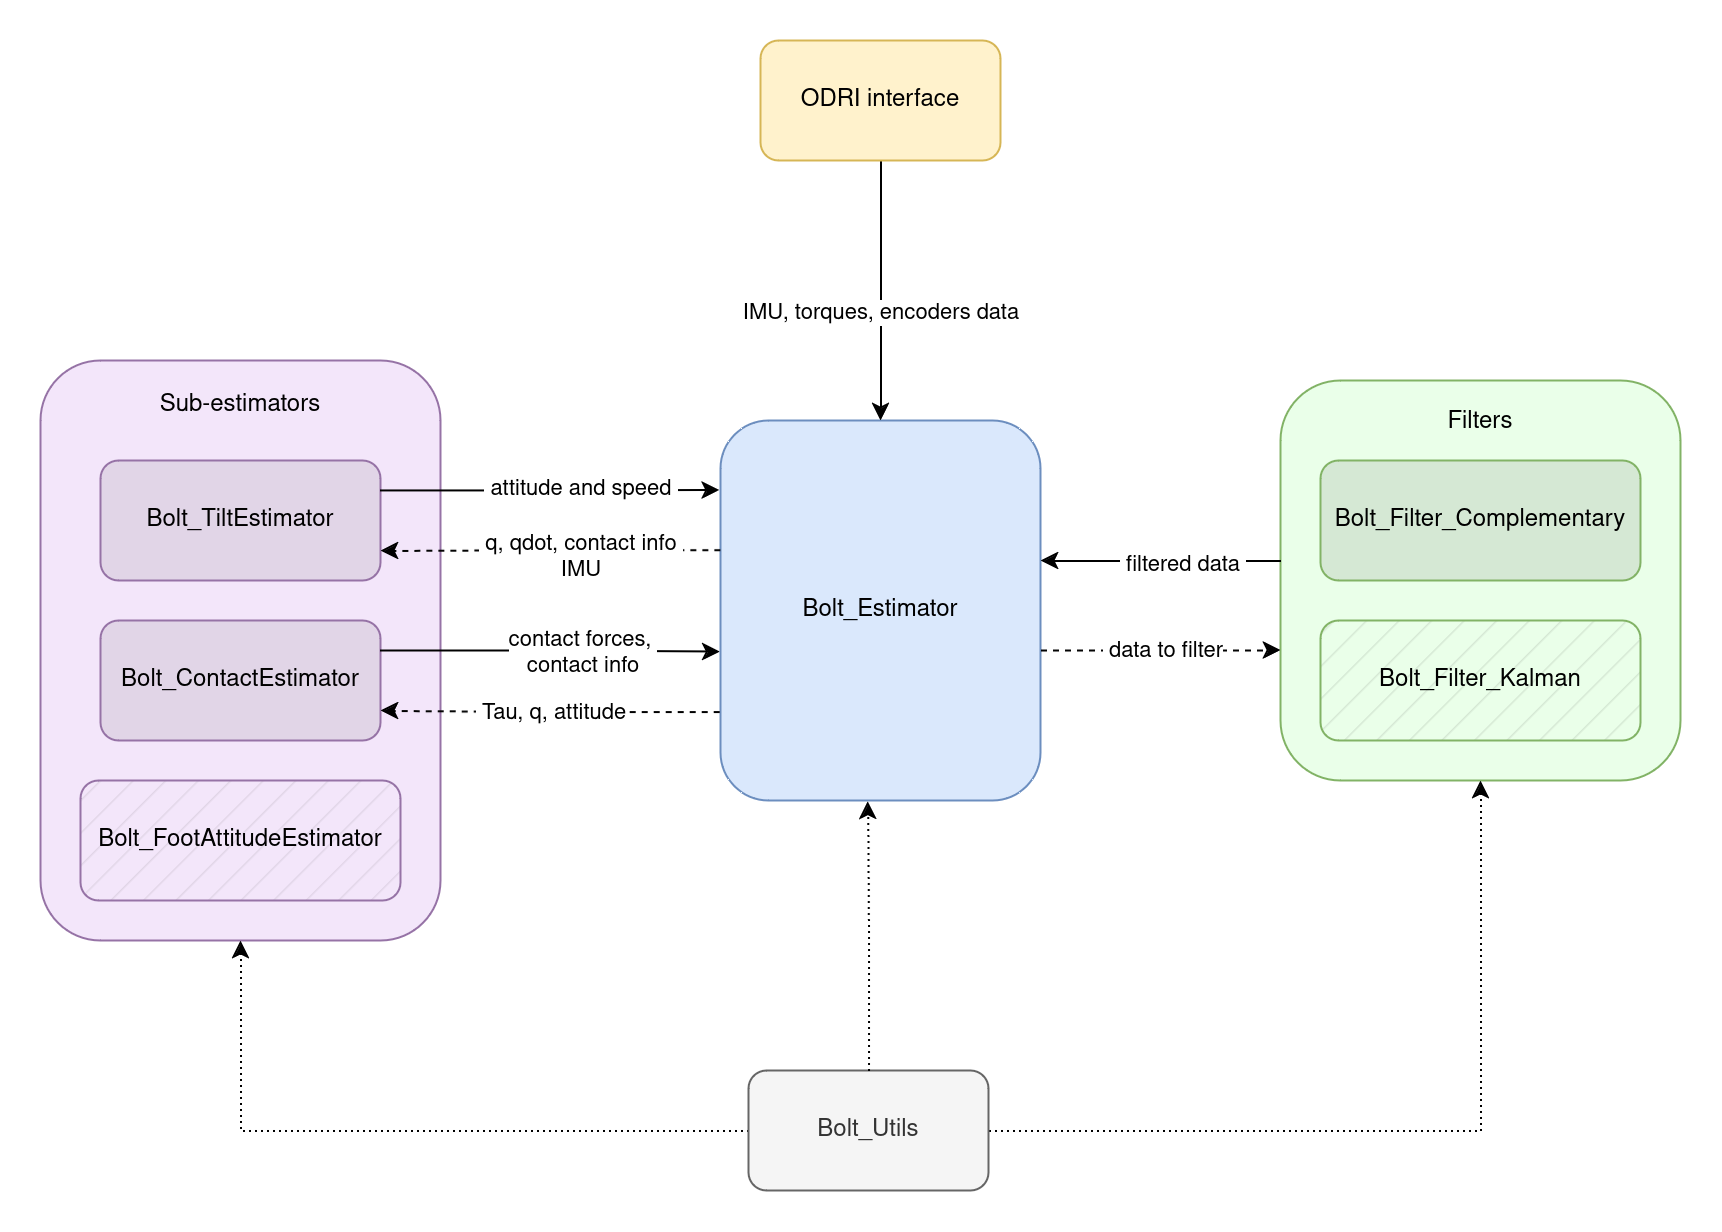
\includegraphics[width=\linewidth, angle=0, scale=1.1]{./images/Structure_simple.png}
  \caption{The structure of Bolt estimator}
\end{figure}

Below is a list of code objects used and an overview of how they interact with one another.

\begin{itemize}
	\item{\textit{Bolt\_Estimator} \\
	Reads the data from sensors, provided by an interface. Initializes and runs filters. Runs \textit{ContactEstimator} and \textit{TiltEstimator}. Merges and filters the obtained data to provide $a$, $\omega$, $c$, ...}
	\item{\textit{Bolt\_ContactEstimator} \\
	Reads data provided by \textit{Bolt\_Estimator}. Derives contact forces on each foot.
	}
	\item{\textit{Bolt\_TiltEstimator} \\
	Reads data provided by \textit{Bolt\_Estimator}. Estimate base attitude and speed in world frame, robot-oriented.
	}
	\item{\textit{Filter\_Complementary} and \textit{Filter\_Kalman} \\
	Filters data provided by estimators or test programs, and returns it.
	}
	\item{\textit{Bolt\_Utils}\\
	Provides a set of objects and functions, such as a logger, to be used in several other objects.
	}
	\item{\textit{TrajectoryGenerator} and \textit{Metal}\\
	Generates a trajectory following user input, with the time derivatives that come with it. It can also read an existing trajectory and derives its time derivatives. It provides a true set and a noisy set of trajectory, speed, acceleration.
	\textit{Metal} adds noise to a provided trajectory.
	}
	\item{\textit{Graphics}\\
	Takes a set of 1D, 2D or 3D trajectories and plots it, with semi-automatic graph settings. }
\end{itemize}

\subsection{Estimator Detailed Architecture}
Below is the Estimator's structure. Compared to previous figure, this one focuses on the Estimator, Contact Estimator and Filter objects. It details their methods. The filters can be of diffent types, such as Bolt\_Filter\_Complementary CITE or Bolt\_Filter\_Kalman.
\begin{figure}[H]
\hspace{-2.5cm} 
%\centering
  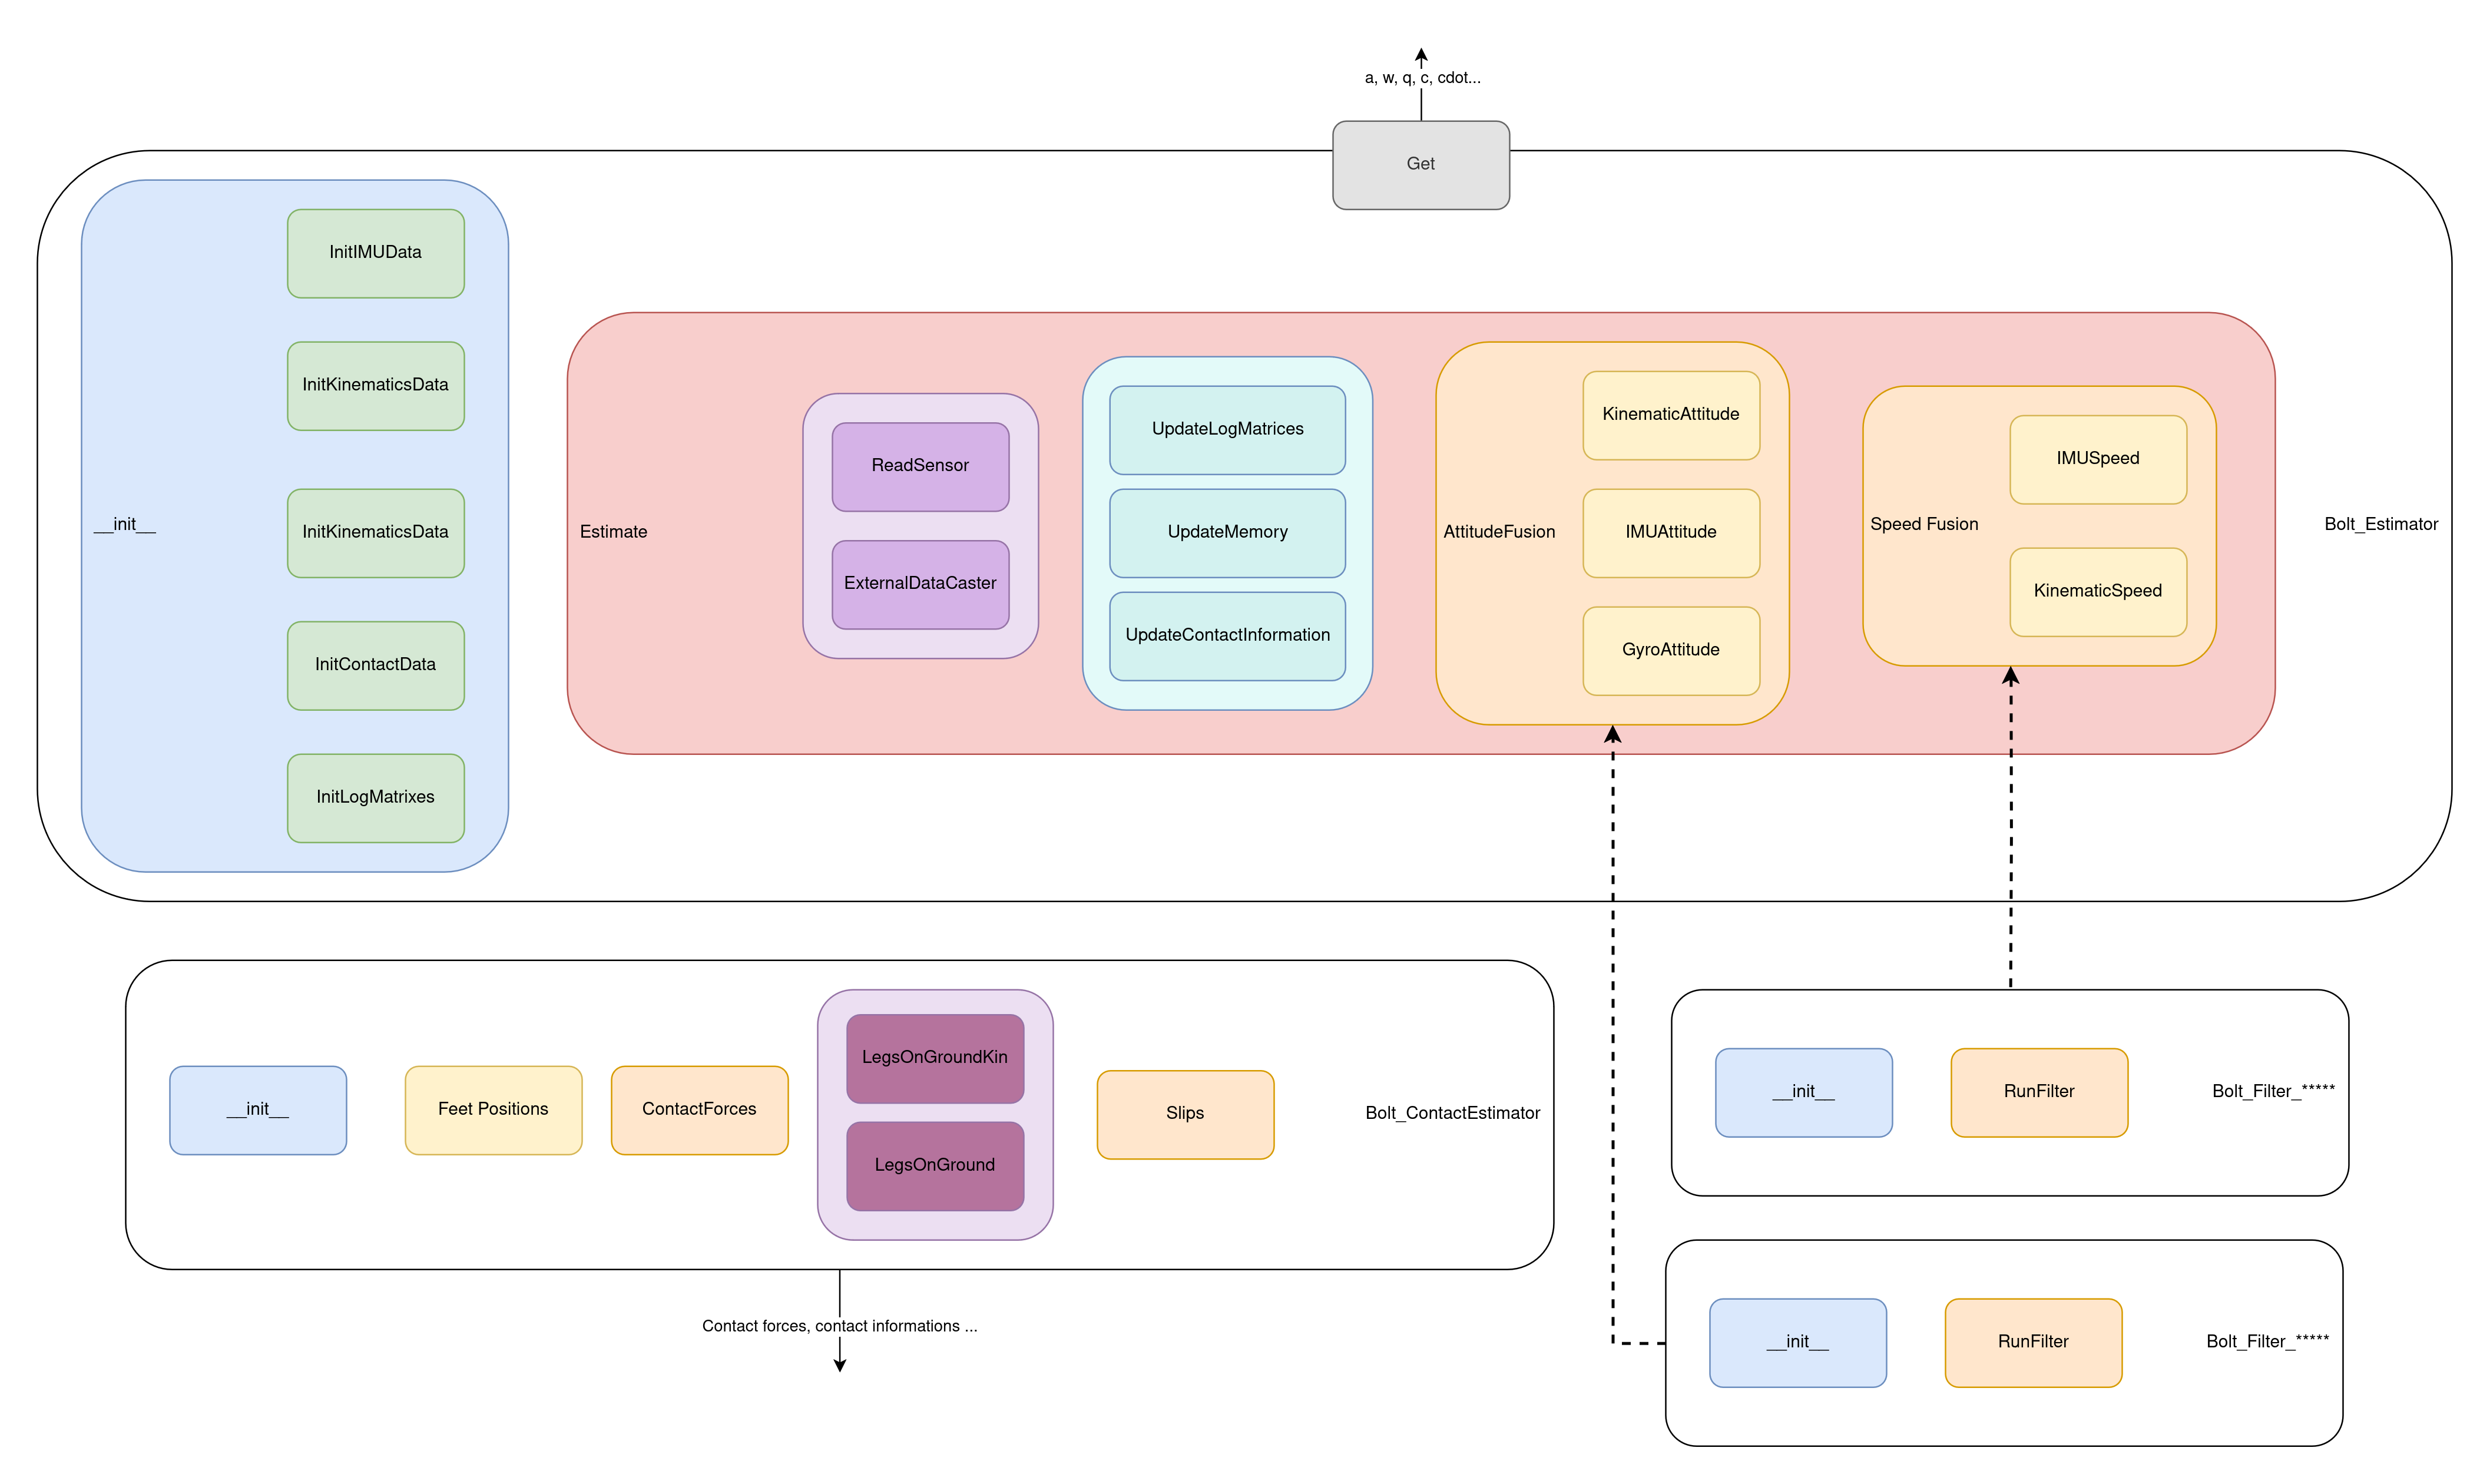
\includegraphics[width=\linewidth, angle=0, scale=1.4]{./images/BoltEstimator0_full_200.png}
  \caption{Estimator architecture \mnaveau{matrices and not matrixes}}
\end{figure}


\section{Filtering}
The proposed estimator needs three distinct filters. These filters might, or might not, have the same specifications and parameters. They are :
\begin{itemize}
	\item{The Attitude filter\\
	uses $\theta_{tilt}$ as quaternion and $\omega_{imu}$\\
	$\hookrightarrow$ gives us $\theta_{filtered}$}
	\item{The Speed filter\\
	uses $a_{imu}$ and $v_{tilt}$\\
	$\hookrightarrow$ gives us $v_{out}$}
	\item{The Base Height filter\\
	uses $v$ and $c$\\
	$\hookrightarrow$ gives us $c_z$}
\end{itemize}
It is of course possible to use one multi-dimensional filter that will do the job of both filters in one go. However, that implies we choose one type of filter for the two different filtering operations. Using 3 different filters proved to be more modular and practical for tuning. \\

\subsection{Filter options comparison}

The best filter we can get for solving this type of problem would be a Kalman filter. It is supposed to be fast and very stable of all \mnaveau{Je comprends pas cette phrase.}. However, Complementary filters are much simpler to tune and provides already accurate results. Solo state-of-the-art estimator is based on a complementary filter. It has to be noted that the 3DM-CX5-AHRS IMU of Bolt and Solo have a built-in Kalman filter, so any filter in our estimator will be added on top of this one. Because it is much simpler to implement and tune, more flexible and has been recommended by both T.Fayols and O.Stasse, the first implemented filter will be a complementary one. Later on, the estimator will offer an array of options for filtering, including at least a Kalman filter and a Complementary filter. To keep this option, Estimator accept filter parameters as list so that the number of parameters can vary depending on the type of used filter.

\subsection{Complementary Filter principle}
\label{complementary filter principle}
In this section :
\begin{itemize}[noitemsep,topsep=0.5pt,parsep=0.1pt,partopsep=0.1pt]
\item $a$ is a frequency in the Laplace domain,
\item $dt$ is a time constant,
\item $x$ is the ground truth signal we want to retrieve from the noisy signal,
\item $x^*$ is the noisy $x$ signal that serves as input,
\item $\widetilde{x}$ is our filter output and estimate for $x$,
\item $c_{og}$ is the integrator / offset gain.

\end{itemize}
A complementary filter (CF) is based on the following scheme \cite{13}:
\begin{figure}[H]
\centering
  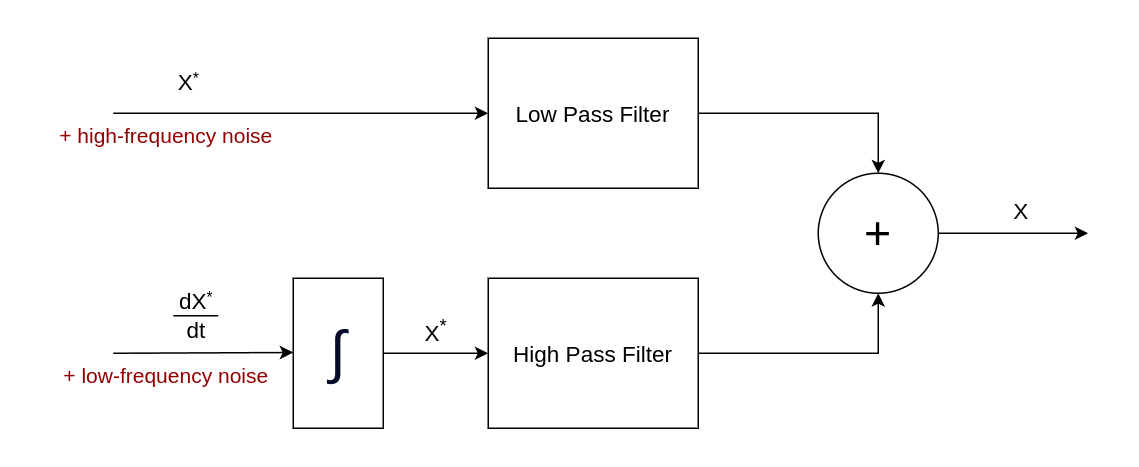
\includegraphics[width=\linewidth, angle=0, scale=0.8]{./images/CF*.png}
  \caption{Complementary Filter}
\end{figure}

We can use first-order low-pass and high-pass filters, whose equations are
$$LP(s) = \frac{1}{1+as}$$
$$HP(s) = \frac{as}{1+as}$$
then
$$\widetilde{x} = \frac{1}{1+as} \cdot x^* + \frac{as}{1+as} \cdot \frac{1}{s} \cdot \dot x^* $$
thus
$$ (1+as) \cdot \tilde{x} = x^* + a\cdot \dot x^*$$
with Laplace inverted transform, we obtain
$$\widetilde{x} + a\cdot \tilde{\dot x} = x^* + a\cdot \dot x^*$$
no longer omitting the time dependance of our functions, we can then approximate $\tilde{\dot x}$ with data we have :
$$\widetilde{x}(t) + a\cdot\frac{\widetilde{x}(t) - \widetilde{x}(t-dt)}{dt} = x^*(t) + a\cdot \dot x^*(t)$$
thus
$$\widetilde{x}(t) = \frac{a}{dt+a}\cdot \widetilde{x}(t-dt) + \frac{dt}{dt+a}\cdot x^*(t) + \frac{dt\, a}{dt+a}\cdot \dot x^*(t) $$

\vspace{4mm}

\noindent denoting $b=\frac{a}{dt+a}$ we get

\vspace{2mm}


$$\widetilde{x}(t) = b\cdot \widetilde{x}(t-dt) + (1-b)\cdot x^*(t) + dt\cdot b\cdot \dot x^*(t) $$
we have the output depending only on inputs and previous outputs.

\bigskip
The parameter $a$ depends on the frequencies of the noise we want to cut, and is often chosen at a few Hz. $dt$ depends on the refresh rate of the filter.
After implementing this filter along with a trajectory generator, here is what we get :

\begin{figure}[H]
\centering
  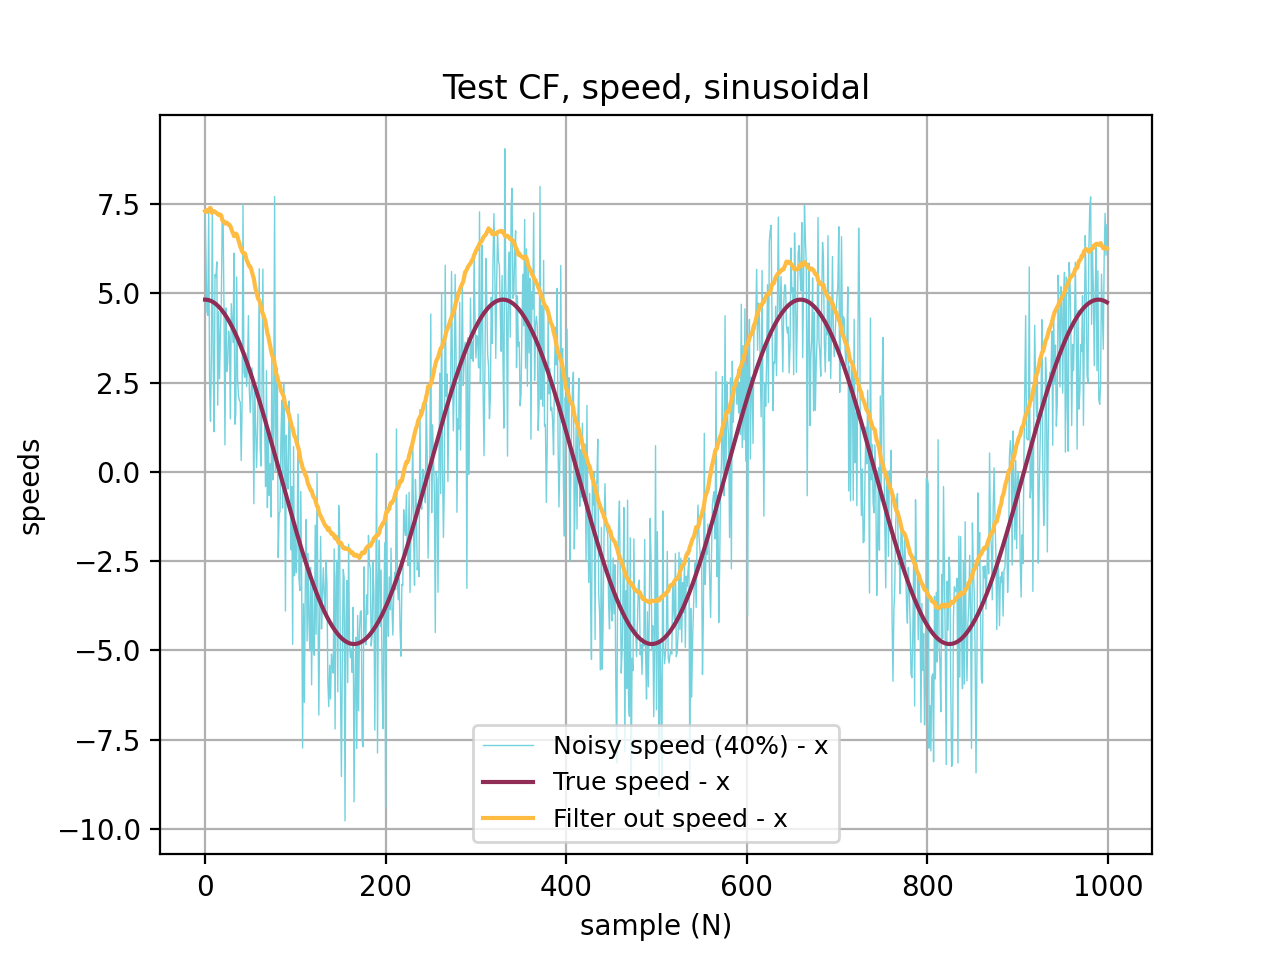
\includegraphics[width=\linewidth, angle=0, scale=0.8]{./images/CF_withoutoffset.png}
  \caption{Simple complementary filter run}
\end{figure}
The generator generate the purple sinus curve and its derivative, corresponding to speed and acceleration. The signals are composed of 1000 points. It then add a white gaussian noise to both. The noisy speed and acceleration is the input of the CF.\\


\subsection{Complementary Filter with integrator}
\label{complementary filter integrator}
It appears that the filter output (yellow) is close enough in shape to the purple targeted signal. However, there is an offset between the signals.
To address this issue, an option is to average the noisy signal and the filter output over $\Delta T$, and consider that the difference between those averages is the offset we want to get rid of. $\Delta T$ has to be chosen long enough for the noise to cancel itself out, and small compared to a characteristic time of the signal. On the following exemples, this $\Delta T$ is arbitrarily set around $0.1$s. This acts as a pseudo-integration of the error.\\
In discrete-time, it changes the output as follows :
$$\widetilde{x}_k \mapsto \widetilde{x}_k + c_{og} \cdot M_k^N$$

where $$M_k^N = \sum_{j=k-N}^{k}\widetilde{x}_j - \sum_{j=k-N}^{k}x_j^* = \sum_{j=k-N}^{k}(\widetilde{x}_j - x_j^*) $$
is the integrated error over the past $N$ samples. 


\begin{figure}[H]
\centering
  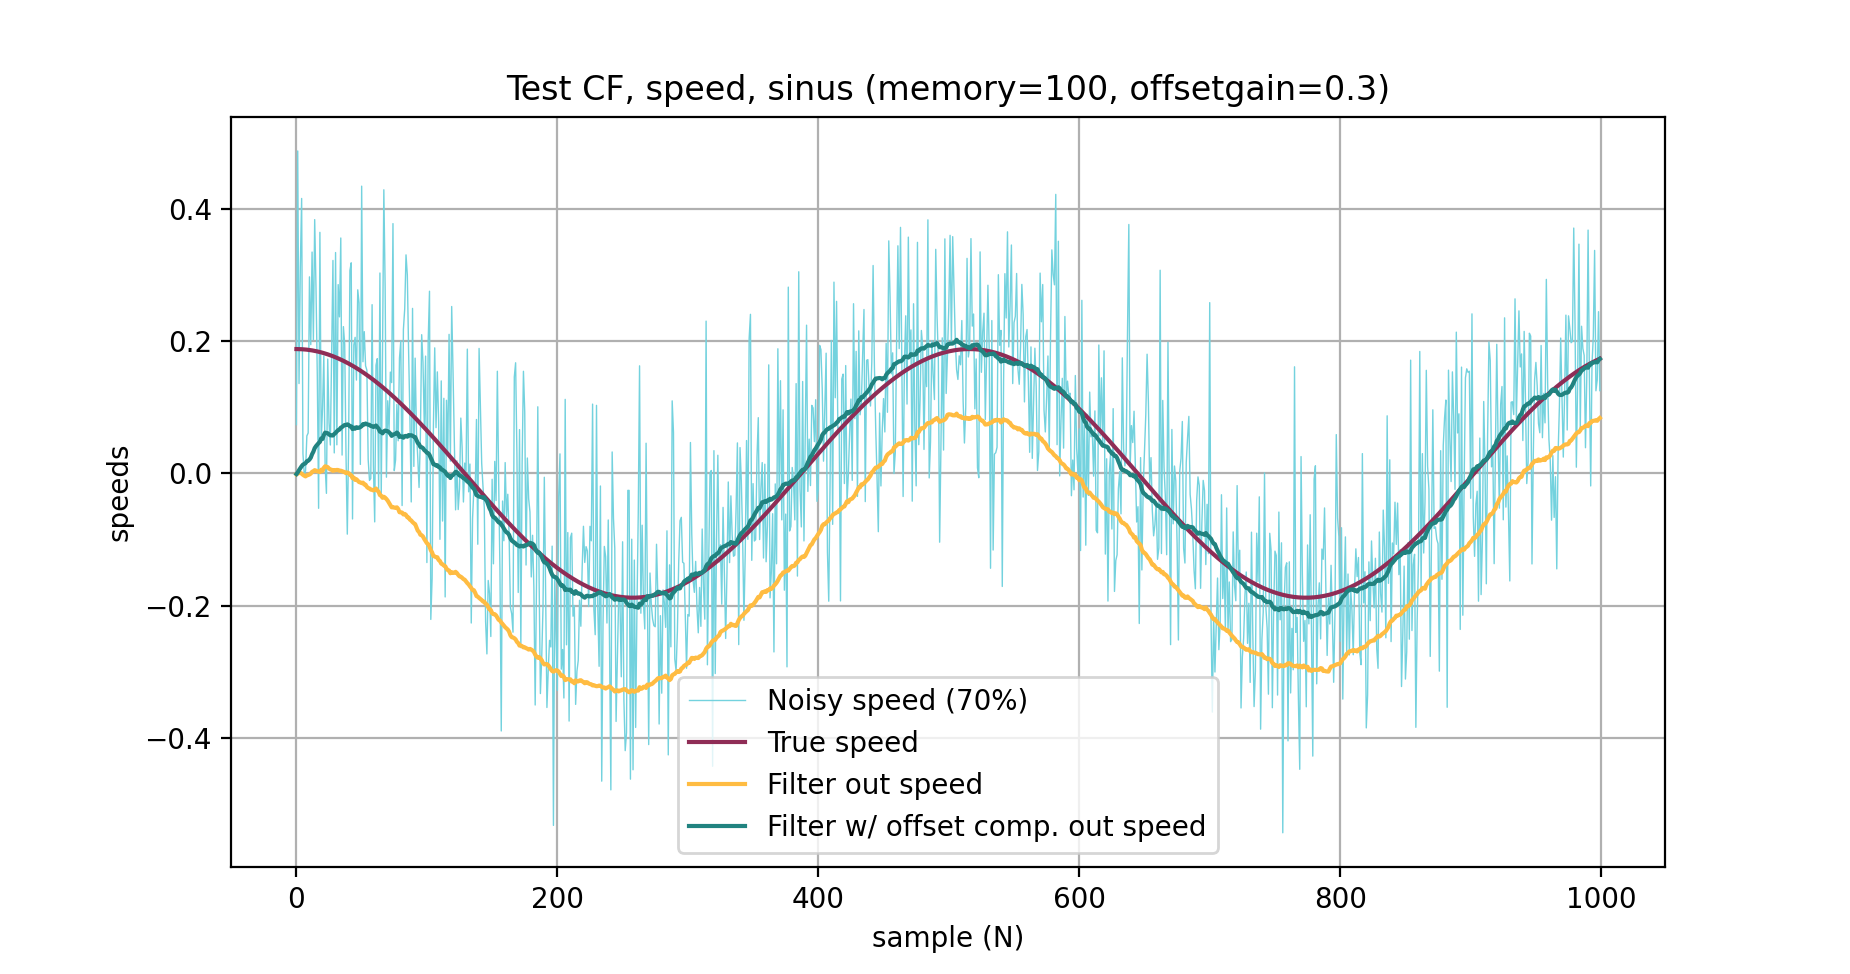
\includegraphics[width=\linewidth, angle=0, scale=0.8]{./images/TestCF_run8_sinus.png}
  \caption{Complementary filter run, with and without offset}
\end{figure}

In most cases, this filter successfully get rid of the unwanted offset. Yet its performances depends a lot on the chosen $\Delta T$. This is most visible on very noisy, slow dynamics polynomial signals. Here, $\Delta T$ ranges from $0.02$s to $0.3$s.

\begin{figure}[H]
\centering
  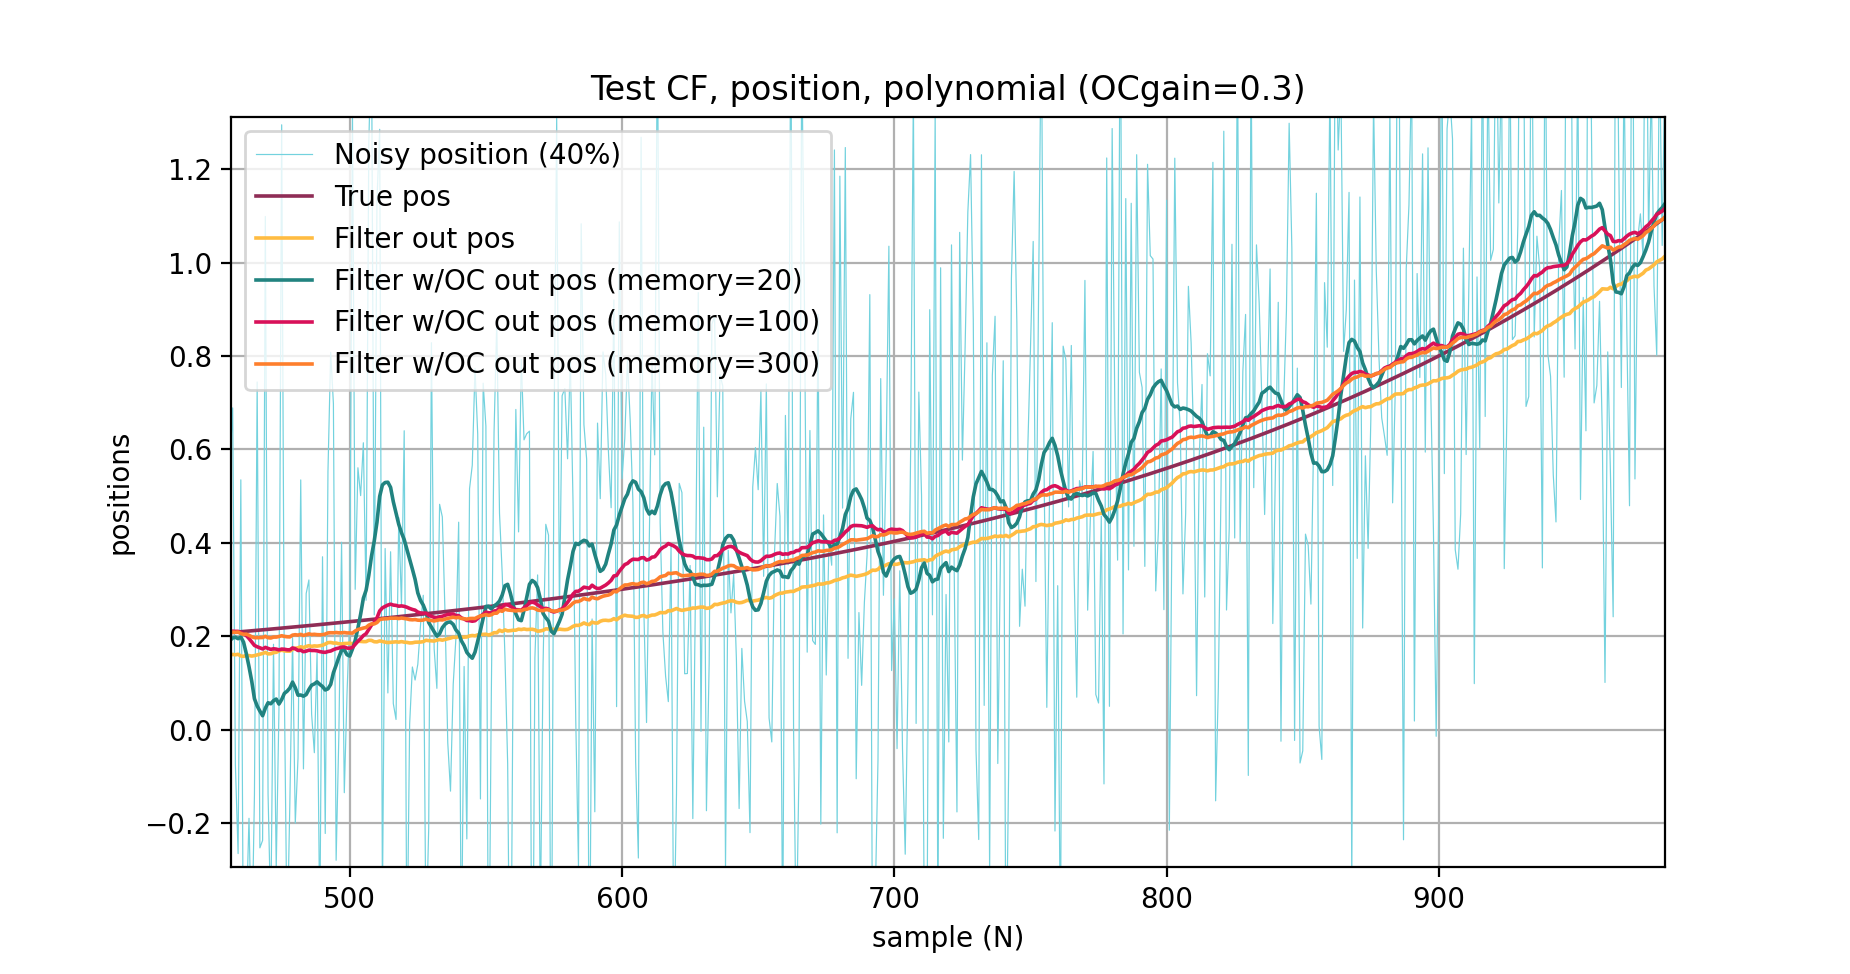
\includegraphics[width=\linewidth, angle=0, scale=1.1]{./images/TestCF_run14_polynomial.png}
  \caption{Complementary filter run, with different memory sizes}
\end{figure}

Still, on some signals, this pseudo-integration takes some time to overcome the bias completely. This time of integration depends on the memory size, but I could not reduce it below around $200$ signal samples without having an noisy filter output. 

\begin{figure}[H]
\centering
  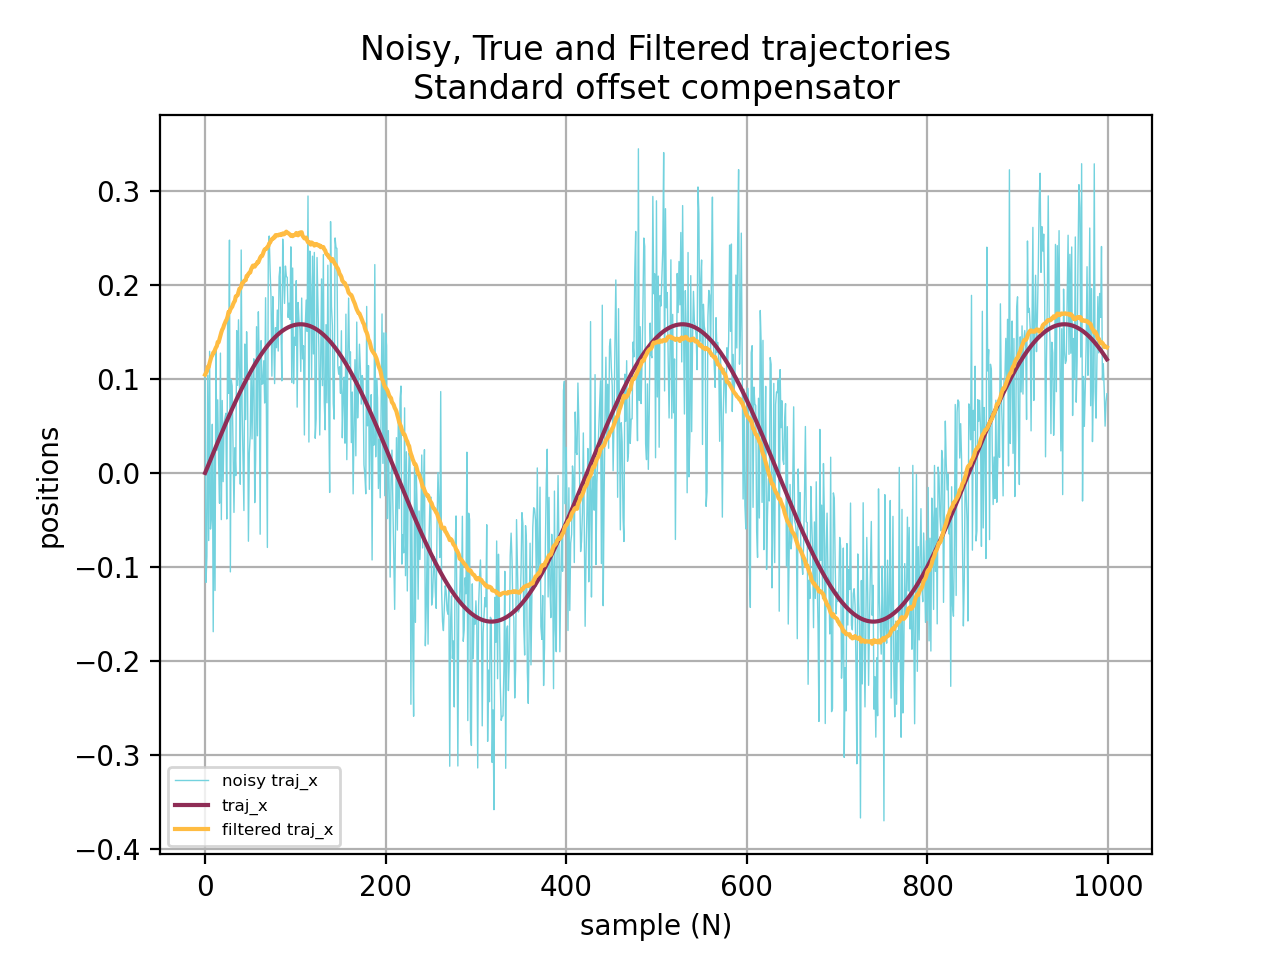
\includegraphics[width=\linewidth, angle=0, scale=0.8]{./images/CF_test_sinus_1_Standard.png}
  \caption{Error integration needs some time to take effect}
\end{figure}


To address this issue, a time-varying gain was implemented. It works as follow.
$$\widetilde{x}_k \mapsto \widetilde{x}_k + c_k^{quickgain} \cdot M_k^N$$
where $M_k^N$ remains the averaged error over the $N$ past samples, and
$$c_k^{quickgain} = max( c_{og} , (\frac{N}{\alpha} - k)\beta) $$
$$\alpha, \beta \in\mathbb{R}$$
It enables quicker convergence on the $\frac{N}{\alpha} - \frac{c_{og}}{\beta}$ first iterations. However, it is sensitive to a non-null average noise on that first period.

\begin{figure}[H]
\centering
  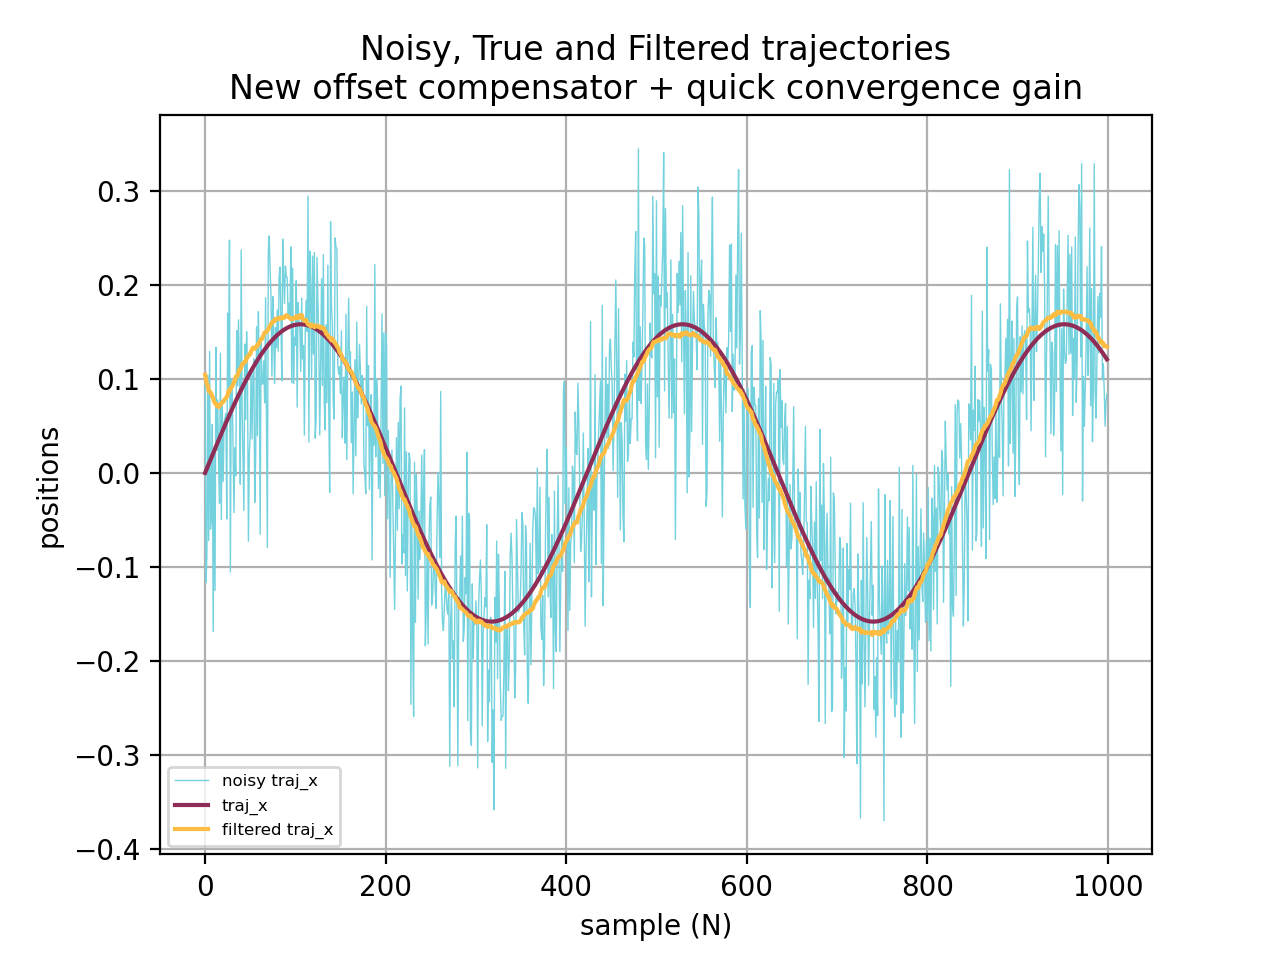
\includegraphics[width=\linewidth, angle=0, scale=0.8]{./images/CF_test_sinus_3_QuickConvGain.png}
  \caption{Same signal as previous figure, but with adaptative gain}
\end{figure}

Let's check that this filter with pseudo-integration is able to perform its function on signals with drifting derivatives.

\begin{figure}[H]
\centering
  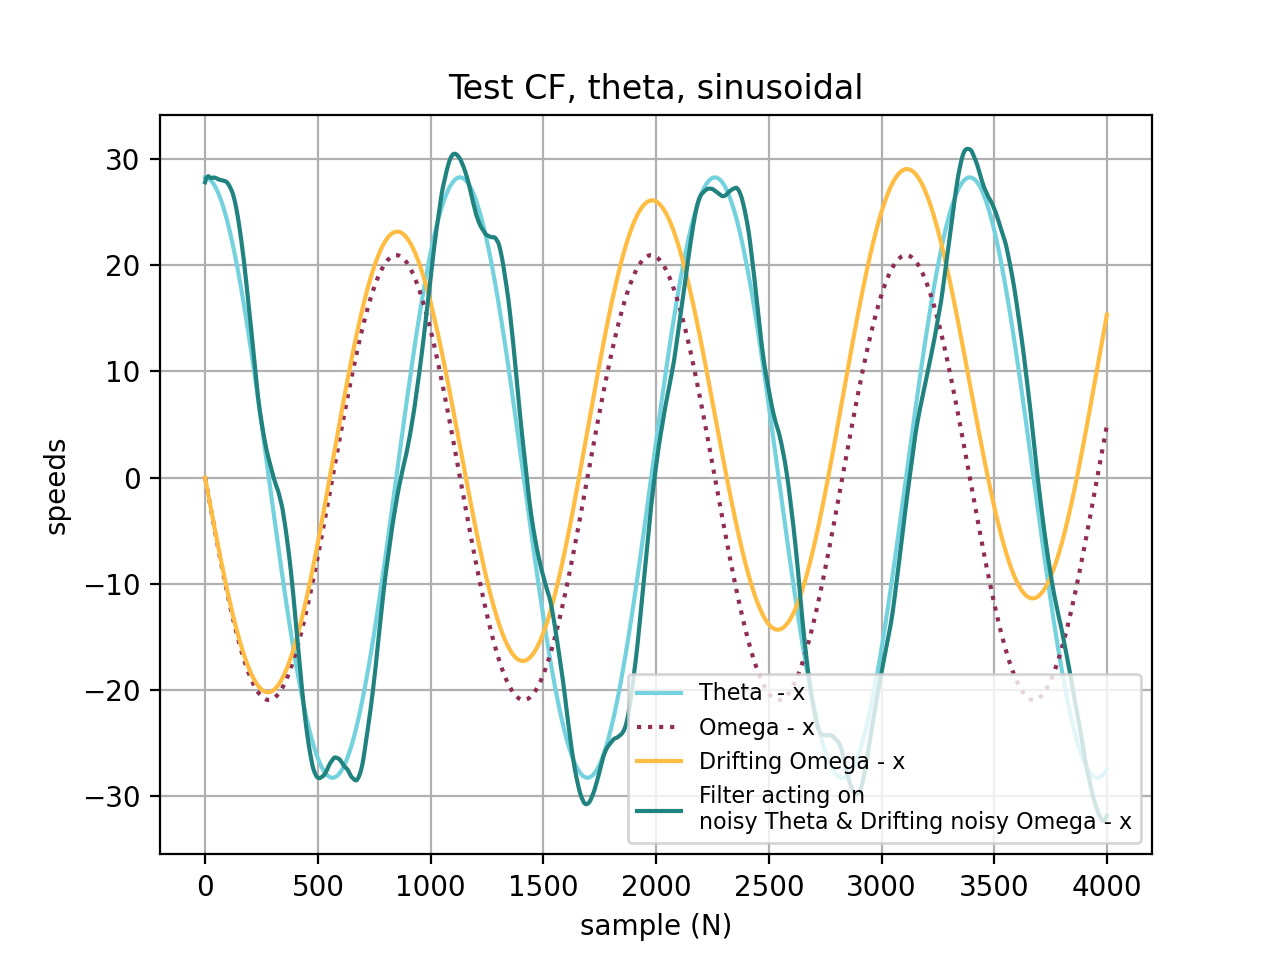
\includegraphics[width=\linewidth, angle=0, scale=0.8]{./images/CF_Drifting_Signal.png}
  \caption{Filter with pseudo-integrator running on a signal with drifting derivatives}
\end{figure}
In this situation, we generate a signal ($\theta$) and its derivative ($\omega$). We then add a drift to $\omega$ : its is no longer a function like $sin(x)$ but rather $x + sin(x)$. On top of that, blank noise is added to both $\theta$ and $\omega$ before they are sent to the filter. This process serves as a simplistic model for IMU data filtering, in which $\omega$ from the accelerometer has a high-frequency noise, but no drift, and $\theta$ from the gyrometer has a drift we have to make up for.


\subsection{Complementary Filter for quaternion}
\label{complementary filter quaternion}
In order to obtain faster computation and prevent singularities, the estimator uses quaternions \cite{4} to describe attitude. However, angular speed are represented by a vector of $\mathbb{R}^3$. From our code point of view,
$$\theta_q \in\mathbb{R}^4$$
$$\omega \in\mathbb{R}^3$$
However, our complementary filter needs $x^*$ and $ \dot x^*$ to be of same dimension. We need to adapt our filter to work properly in this situation.

\medskip
We denote
$$\theta_q = \begin{bmatrix}  q_x\\ q_y\\ q_z\\  q_{\omega}      \end{bmatrix}$$
$$\omega = \begin{bmatrix}  \omega_x\\ \omega_y\\ \omega_z\\    \end{bmatrix}$$

And we filter $\theta_q$ with its time derivative CITE
$$ \dot \theta_q = \omega_q = 0.5 \cdot \begin{bmatrix}  
 0 \hspace{15pt}  -  \omega_x q_x    -   \omega_y q_y   -   \omega_z q_z\\
\omega_x q_\omega + \hspace{7pt} 0 \hspace{7pt} + \omega_z q_y - \omega_y q_z\\
\omega_y q_\omega - \omega_z q_x + \hspace{7pt} 0 \hspace{7pt} + \omega_x q_z \\   
\omega_z q_\omega - \omega_y q_x - \omega_x q_y + \hspace{15pt} 0 \\   

    \end{bmatrix} \hspace{15pt} \in\mathbb{R}^4$$
with the exact same method described in \ref{complementary filter principle}, with $x^* = \theta_q$ and $ \dot x^* = \omega_q$ of dimension $4$.

\subsection{Implementation of complementary filter}

\mnaveau{TODO: Add the link to the code.}

As \ref{complementary filter integrator} and \ref{complementary filter quaternion} explained different modifications of the filtering process, these are implemented in the \textit{Bolt\_Filter\_Complementary} class. Below are the method to run the filter from which to chose.

\begin{itemize}
	\item Runfilter : run the filter
	\item RunFilterQuaternion : run the filter on a quaternion and an angular speed
	\item RunFilterOffset : run the filter with a pseudo-integrator
	\item RunFilterOffsetAdaptative : run the filter with a pseudo-integrator and a stronger gain in the first iterations
\end{itemize}

A \textit{Bolt\_Filter\_Complementary} object keeps its last estimate as a state variables and store various logs. It necessary that a given filter is used always on the same data, for instance not on speed and then on attitude. 


\section{Estimating Tilt and speed}
\label{estimating tilt and speed}

\subsection{Goals}
The IMU provides us the sum of earth's gravity and robot's base acceleration. From this sum, we want to obtain the direction of earth's gravity, and from this direction we can derive the attitude of the robot'base. Additionally, the IMU includes a gyrometer which gives us access to the first-order time derivative of the attitude. This is suitable for a complementary filter implementation.\\
The objective is to reconstruct the attitude of the robot's base based on all this. 

\subsection{Implementation}
\mnaveau{Dans le .bib tu ne devrais pas noter les papier avec des numeros. Tout l'interet de ce fichier c'est d'avoir une system intelligible. Je te modifie le CITE suivant pour te montrer.}
The code used is an implementation of \cite{Benallegue_2020}
The code file is named Bolt\_TiltEstimator and is composed of functions:
\begin{itemize}
	\item{init}
	\item{InitLogs and UpdateLogs\\Can be disabled.}
	\item{SetInitValue function\\ It enables one to change the start truth to prevent bias due to initial conditions.}
	\item{PinocchioUpdate\\This function centralize all calls to Pinocchio. It updates every data from Pinocchio that might be used during computation. For instance, it updates the attitude and speed of the base in contact foot frame.}
	\item{ErrorUpdate\\ Update an estimate of the errors on state variables as they were defined in the paper. Not used elsewhere in the code.}
	\item{Estimate\\This is the main function. It calls PinocchioUpdate, compute the state variable derivative, and integrate them. It then returns the state variables.}
\end{itemize}

Please note :\\

\begin{itemize}[noitemsep,topsep=0.5pt,parsep=0.1pt,partopsep=0.1pt]
	\item{This function needs to know which foot is touching the ground. It relies on contact information provided by Estimator.}
	\item{Logging can be disabled for less memory use and faster processing.}
	\item{Notation are the same as those used in the paper.\\ $x_1$ is the speed, $x_2$ is a unite vector corresponding to the gravity direction.}
	\item{Two possibilities are mentionned by the author (in a yet to come update of the paper) to compute $y_v$. \mnaveau{I don't get what is $y_v$ here.} Both are implemented, only the first one is used.}
	
\end{itemize}

Fig.\ref{fig:speed_datapipe} and Fig.\ref{fig:tilt_datapipe} are schemes about the implementation of tilt and speed estimation.

\begin{figure}[H]
\centering
  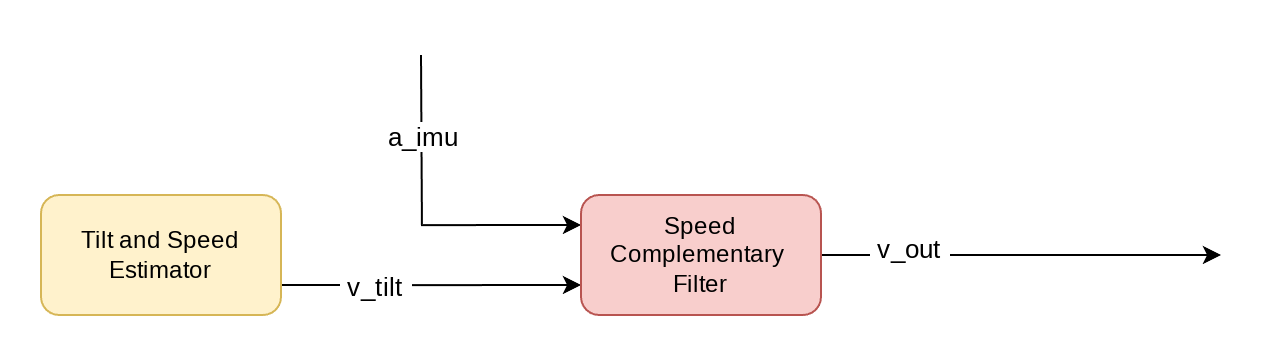
\includegraphics[width=0.9\linewidth]{./images/Variable_Speed.png}
  \caption{Speed datapipe}
  \label{fig:speed_datapipe}
\end{figure}

\begin{figure}[H]
\centering
  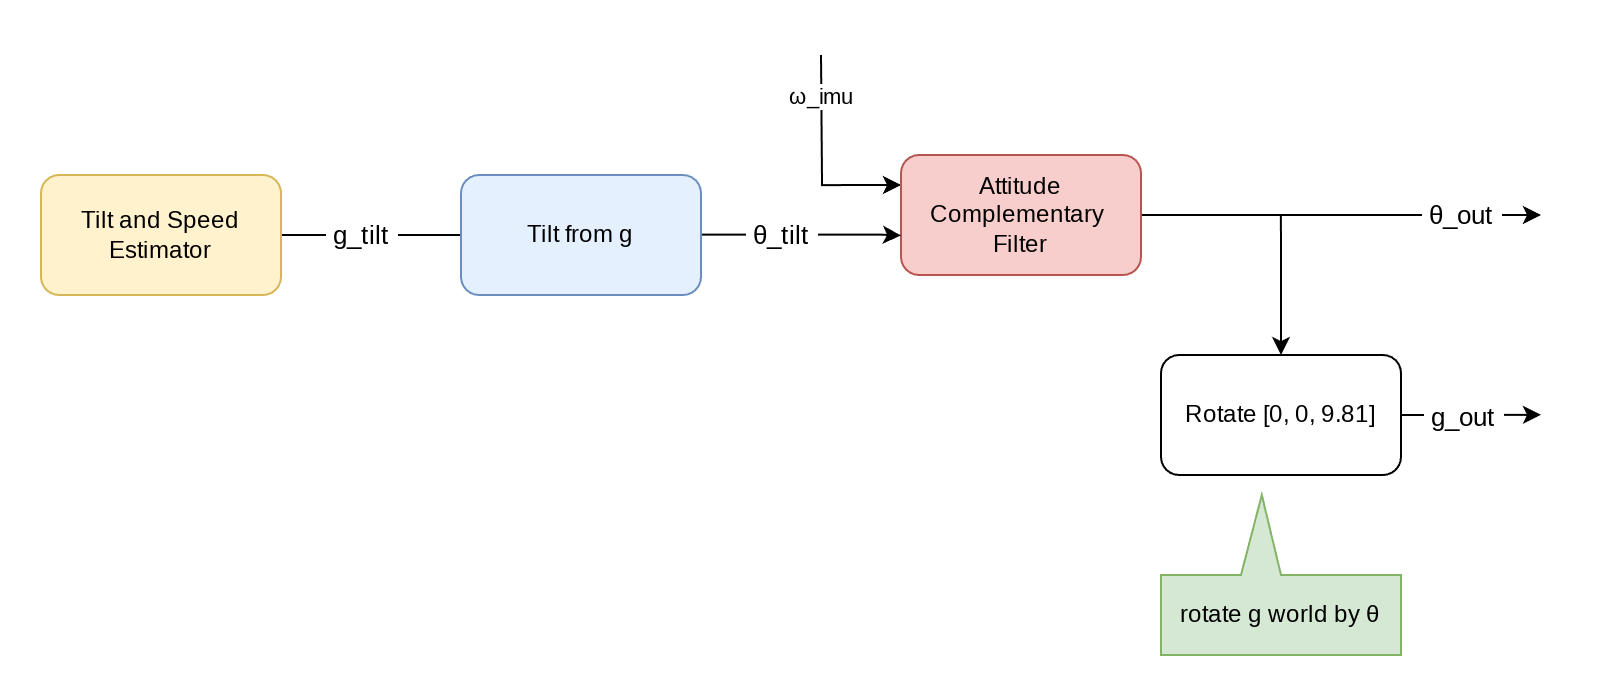
\includegraphics[width=\linewidth]{./images/Variable_Attitude.png}
  \caption{Tilt datapipe}
  \label{fig:tilt_datapipe}
\end{figure}


\section{Estimating Contacts}
\subsection{Goals}
Bolt does not have force sensors in its feet. Therefore, Bolt doesn't know wether or not it is touching the ground. Moreover, it has no way of knowing the angle its rounded feet make with the ground. Knowing this can prove useful to correct or complete attitude measurements.

\subsection{Structure}
To estimate wether or not a foot is touching the ground, we proceed as follow.
\begin{enumerate}[noitemsep,topsep=0.5pt,parsep=0.1pt,partopsep=0.1pt]
	\item Estimate the contact forces from legs torques, IMU acceleration, model dynamics. That gives us 3 different estimates.
	\item Check that these forces are trustworthy (eg, coherent with one another).
	\item Consider that the stronger the contact force, the most likely our contact is.
	\item Return a boolean value based on the trust and the probability
\end{enumerate}


\begin{figure}[H]
\centering
  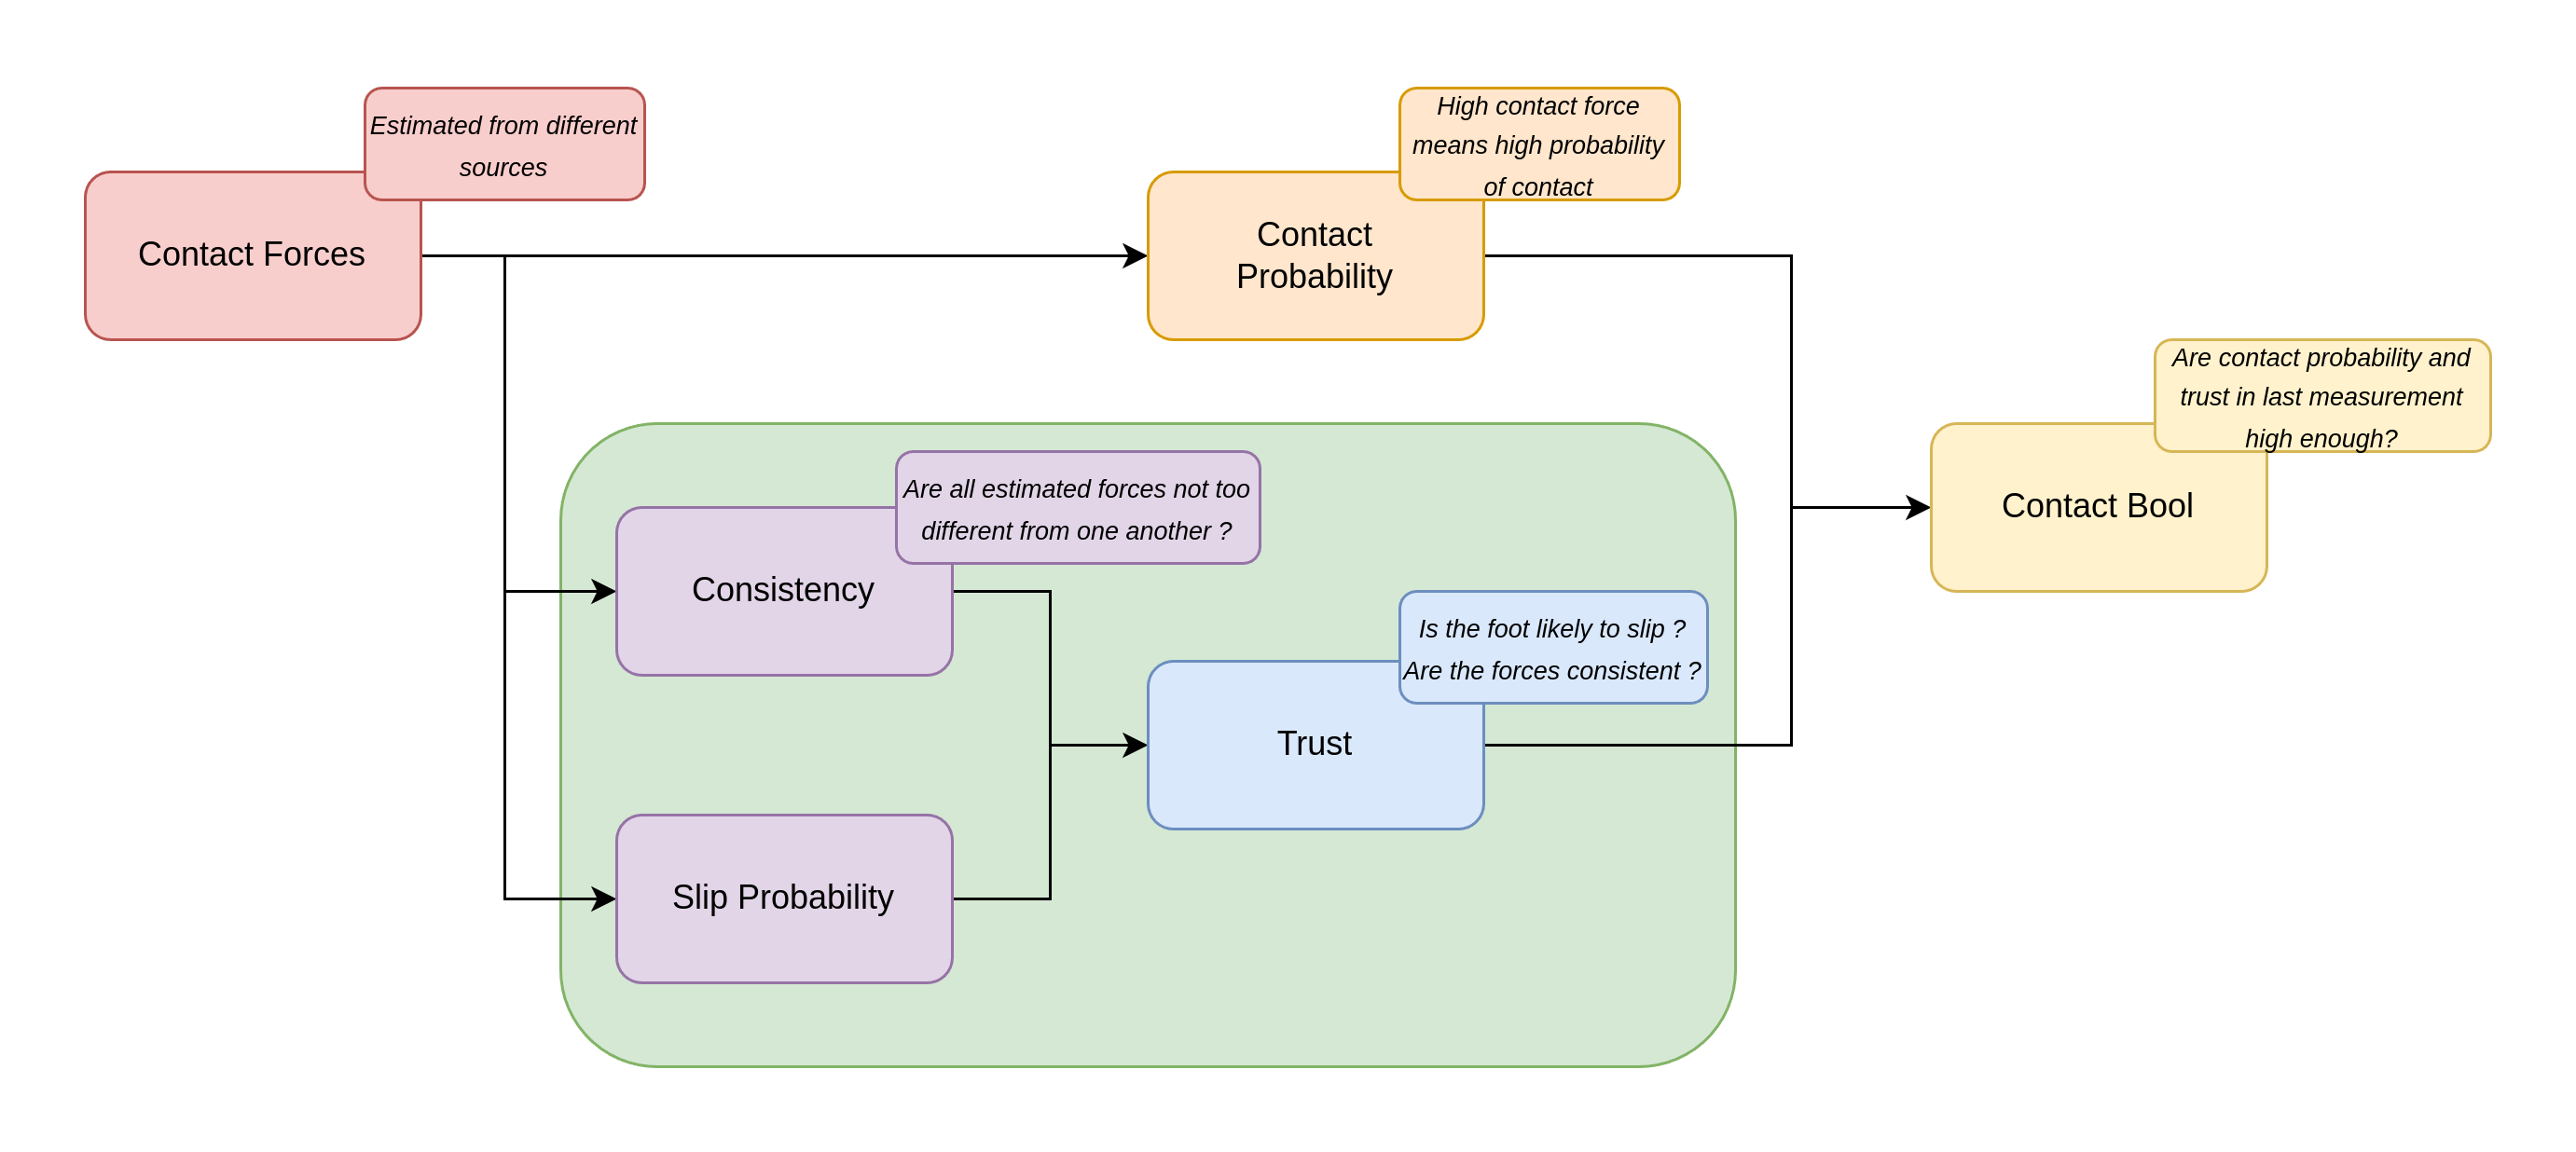
\includegraphics[width=\linewidth, angle=0, scale=1.2]{./images/Logique_ContactEstimator.png}
  \caption{How ContactEstimator works}
\end{figure}




\subsection{Contact Forces}
We have different ways of estimating contact forces \cite{6}\cite{10}\cite{14}. The implemented methods are as follow :

\begin{itemize}
	\item ContactForce1D : Estimate the contact force on both feet.\\
	It considers that contact forces $F_1, F_2$ are vertical (which is untrue), each applied at the center of a foot (which should be close from true). Then, it considers that 
	$$F_1, F_2 = \argmin_{F_1, F_2}(\ddot c_{imu} - \ddot c_{fk}(F_1, F_2, \tau, \dot q))$$
	We obtain $F_i^{1D} = \begin{bmatrix}0\\ 0\\ F_i^z \end{bmatrix}$ 
	\item ContactForce3D : Estimate the contact force on both feet.\\
	It uses the fact that if one neglect the legs inertia and speed \cite{9} \cite{10}, one has 
	$$ F_c = (J_c^T)^{-1} \cdot(\tau - b - g)$$
	$b$ being the nonlinear term and $g$ the generalized gravity.
	\item ContactProbability\_Torque : Estimate the contact force and contact probability on both feet.\\
	This function is simple and takes advantage of the geometry of Bolt. We use the attitude estimate and the encoders to compute the horizontal knee-foot distance $d$. Then, we divide the knee torque by $d$. We thus obtain the contact force.
	\begin{figure}[H]
	\centering
  	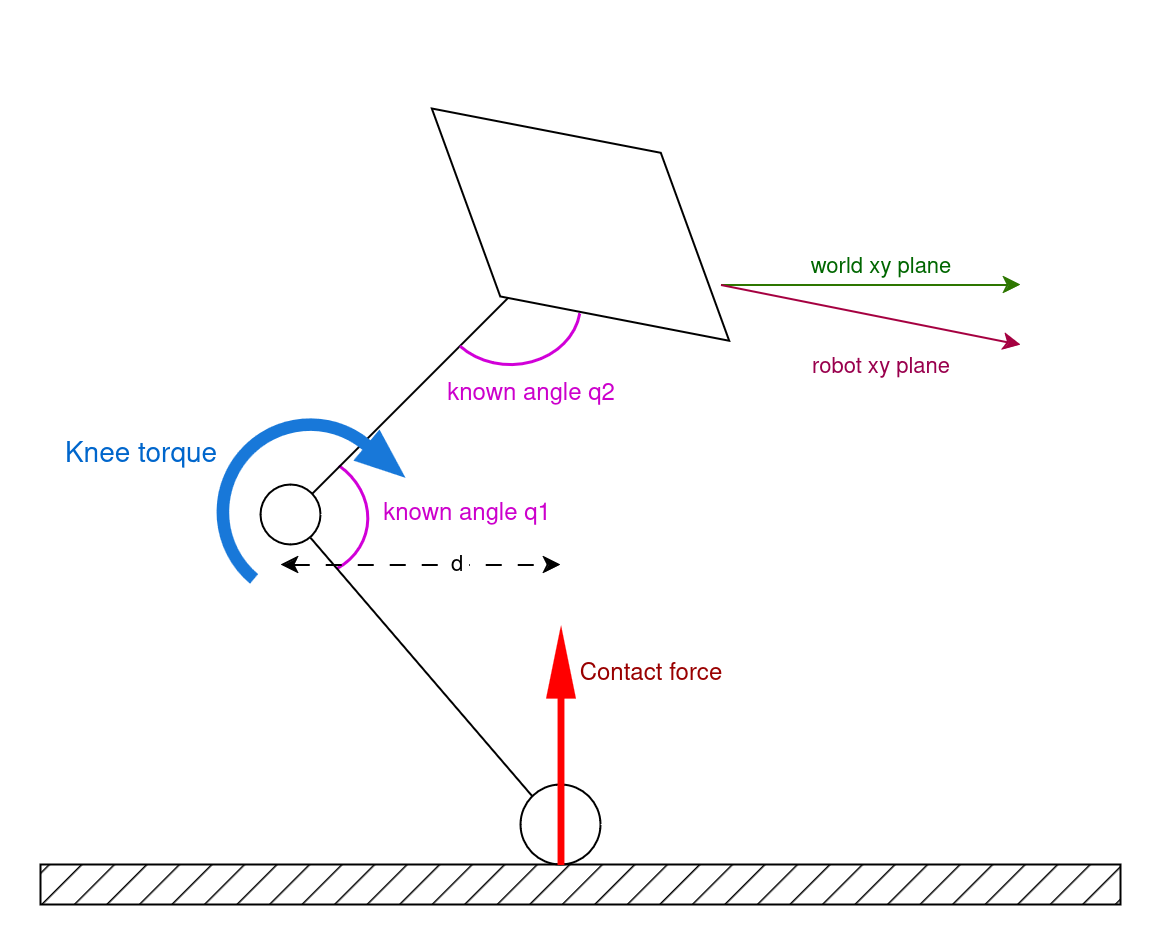
\includegraphics[width=\linewidth, angle=0, scale=0.5]{./images/Bolt_KneeTorque.png}
  	\caption{Contact probability using knee torque only}
	\end{figure}
	
\end{itemize}

At this point, we have different estimates for our contact forces. We then introduce a sigmoid probability function as follows :

\begin{align*}
  P_s : \mathbb{R}_+ &\rightarrow [0; 1]\\
  x &\mapsto \frac{1}{1 + e^{-b \cdot x + b_0}} \hspace{1cm} b, b_0  \in\mathbb{R}_+^*
\end{align*}
Which maps any real data to a $[0; 1]$ interval of probability.
And considering that
\begin{align*}
	P_s(x_{center}) = \nicefrac{1}{2} \hspace{3mm} &\Leftrightarrow \frac{1}{2} = \frac{1}{1 + e^{-b \cdot x_{center} + b_0}}\\
						&\Leftrightarrow 1  =e^{-b \cdot x_{center} + b_0}\\
						&\Leftrightarrow b\cdot x_{center} = b_0
\end{align*}

we will tune the parameters $x_{center}$ and $b_0$ by hand, and compute $b$ such that $P_s(x_{center}) = \nicefrac{1}{2} $, ie
$$b = \frac{b_0}{x_{center}}$$

\begin{figure}[H]
\centering
  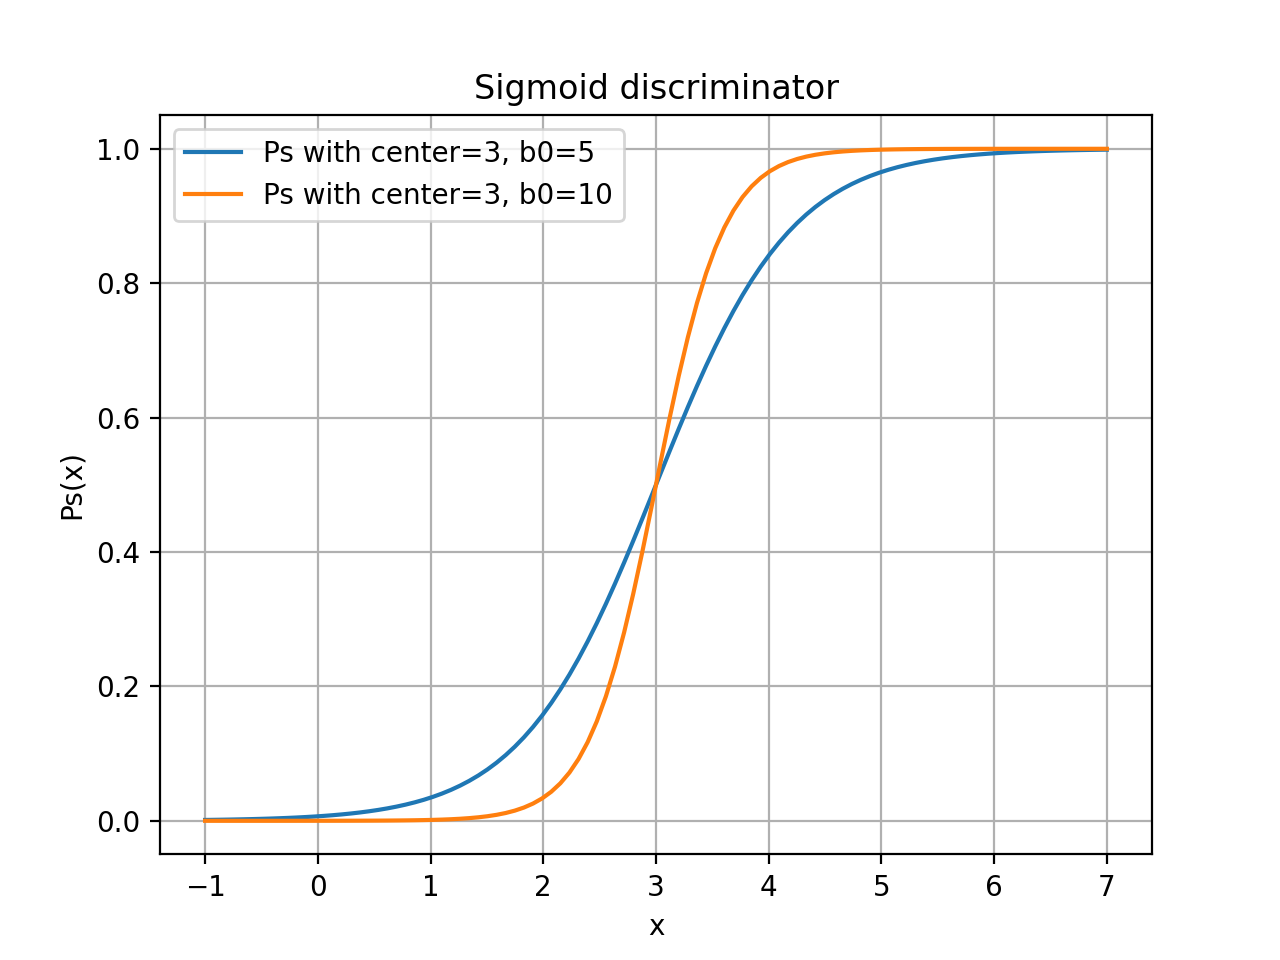
\includegraphics[width=\linewidth, angle=0, scale=0.8]{./images/ProbDisc_1.png}
  \caption{The $P_s$ function centered on $3$ with different stiffnesses. \mnaveau{Oublie pas les "." a la fin des phrases. Si possible utilise un logiciel pour generer des graphes latex (en general il genere un ".tikz"). Ca te fais des graphes vectoriel et donc zoomable a l'infini. C'est plutot mieux.}}
\end{figure}

Let's suppose one has a measurement $x$ that tells one something about an event $A$. This function gives one an interval $[x_0, x_1]$ where $A$ is almost-impossible, and an interval $[x_2, x_3]$ where $A$ is almost-certain.\\
This can be useful to maps values of torques or contact forces to a probability of contact.

\begin{figure}[H]
\centering
  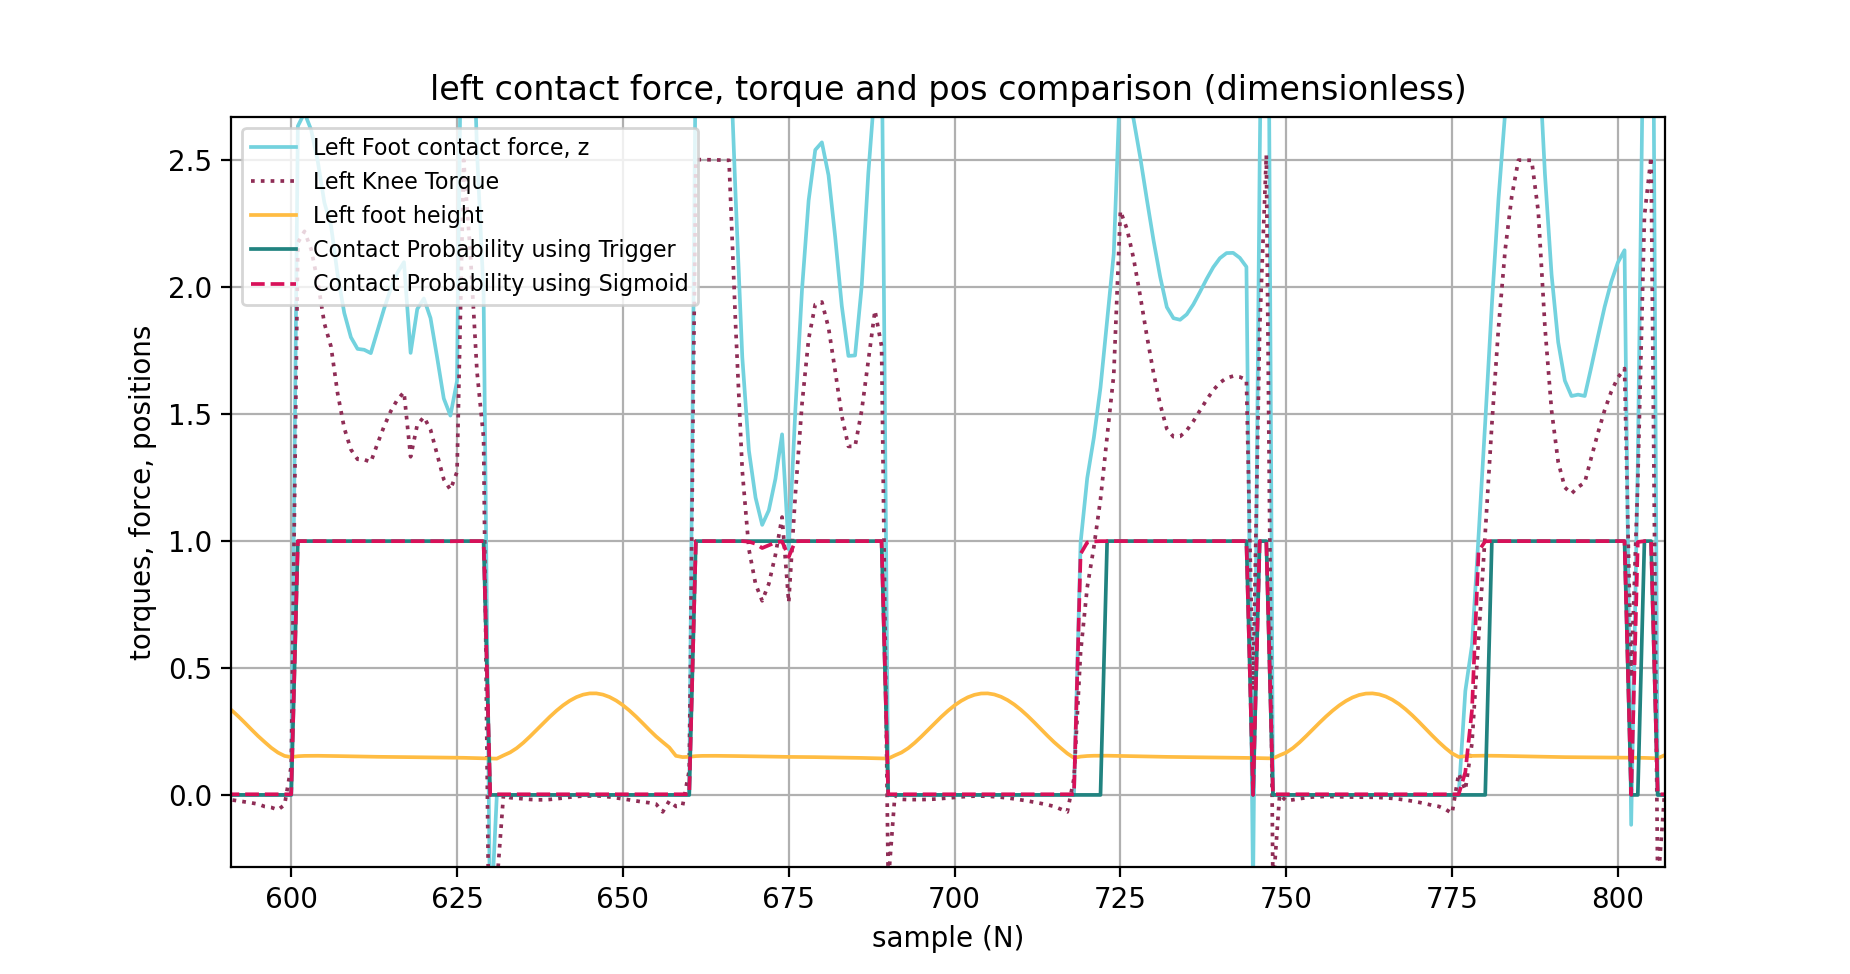
\includegraphics[width=\linewidth, angle=0, scale=1.0]{./images/Torque_Contact_Detection_Comp_difficile.png}
  \caption{Using the $P_s$ function to detect ground contact, using contact force. \\ It proves to be more precise and reactive than a detection using upper and lower trigger.}
\end{figure}



\subsection{Slipping}
For a contact force $F_i^{3D} = \begin{bmatrix}F_i^x\\ F_i^y\\ F_i^z \end{bmatrix}$  we consider the coefficient CITE
$$\mu = \frac{\sqrt{ {F_i^x}^{2} + {F_i^y}^{2}}}{F_i^z} $$
Then, $\mu < \mu_{thresold}$ gives us a criteria about the foot's likeliness to slip. This coefficient is used in \cite{9}. 
Other criterias are the foot's horizontal speed and the foot's horizontal acceleration. 
Each of these coefficients is composed by the $P_s$ function to discriminate cases.


\subsection{Detecting Switches}
Switches denote the moment when the robot changes its stance foot. For instance, the switch can be when the left foot touches the ground, followed shortly afterward by the right foot moving up.\\
The robot can have both of its feet in contact with the ground for some time. This gait is called double support. It might also lift its foot at the exact same time the swing foot touches the ground. This gait is called simple support. In both case, the estimation of contact is not perfect especially around switch times, so there might be unwanted contact detection. To accurately detect the switches, we proceed as follow : 
\begin{algorithm}[htb]
  \caption{Basic switch detection}
  \begin{enumerate}
    \item
    Initialize $Contact Status$ and robot state as not $Switching$.

    \item
    While $True$:
    \begin{enumerate}
      \item
      If a change is detected in $Contact Status$ and robot is not $Switching$\\
      $\hookrightarrow$ robot is now $Switching$

      \item
      If robot is $Switching$\\
      $\hookrightarrow$ do what needs to be done (such as computing feet positions)

      \item
      If two changes are detected in $Contact Status$ \\
      $\hookrightarrow$ swing foot and stance foot have exchanged roles. Robot is no longer $Switching$.
    \end{enumerate}
  \end{enumerate}
\end{algorithm}
To prevent a switch from lasting forever in case of a wrong initialization, a switch timeout is added to this algorithm.

\section{Estimating Position}

\subsection{Goal}
In order to compute the DCM, one needs the position and speed of the center of mass of the robot. These can be inferred from the position and speed of the robot's base. We have estimated the speed in \ref{estimating tilt and speed}, we now need to estimate the position.

\subsection{Principle}
Bolt is a blind robot : it does not have absolute odometry, through Lidar or vision for instance. Our first option is then to integrate the acceleration from the IMU two times :
$$ p_{imu} = \iint_t a_{imu} \, \mathrm{d}t $$
But this is of course drifting very quickly because of noise in $a_{imu}$ and numerical integration errors. It can only provide accurate position estimate for a very short period of time.\\
\newline
Another way is to integrate the previously estimated speed.
$$ p_{inter} = \int_t v_{out} \, \mathrm{d}t $$
This will also drift after a few seconds, because of errors in estimate and numerical integration errors. Yet, it provides a much improved estimate of $p$.\\
\newline
A third way is to sum the length of a footstep. For a very short period of time, every time Bolt puts a new foot on the ground and lift the other, it has its two feet on the ground. We call that a \textit{switch}. During this period, we assume both feet are at a standstill. The distance between the two feet in contact with the ground can then be computed thanks to the encoders data. We thus obtain the length of a footstep.

\begin{figure}[H]
\centering
  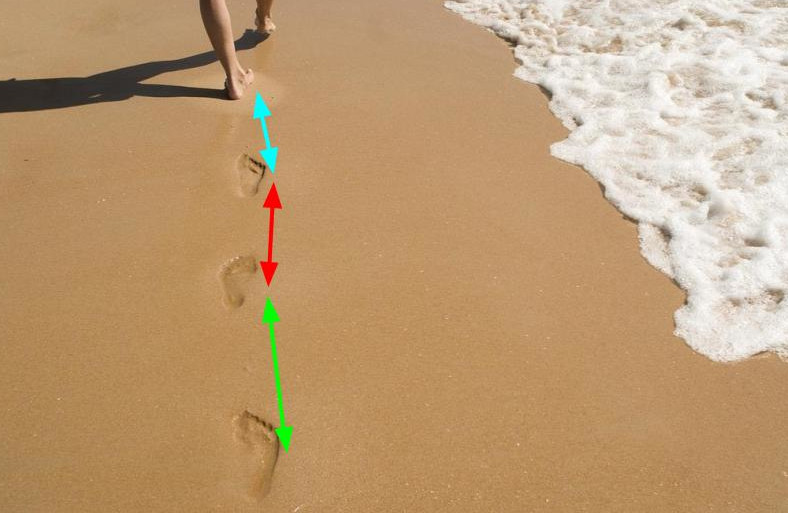
\includegraphics[width=\linewidth, angle=0, scale=0.6]{./images/footprint.jpg}
  \caption{Switch odometry}
\end{figure}

One can see that adding the footstep lengths provides the position of the walker with regards to its starting position. This can be used to compensate the drift of the previous methods, by providing a close estimate of the robot position every footstep.


In the Fig.\ref{fig:XXXX} below one can see the result of switch odometry on a simulation of Bolt. The estimator ran at $1$kHz for $4$ seconds. One can see that footsteps and switches were accurately detected. The shift in $y$ position is due to the alternance between left foot and right foot, and that could be corrected easily. The $z$ estimate however is drifting. 



\begin{figure}[H]
\centering
  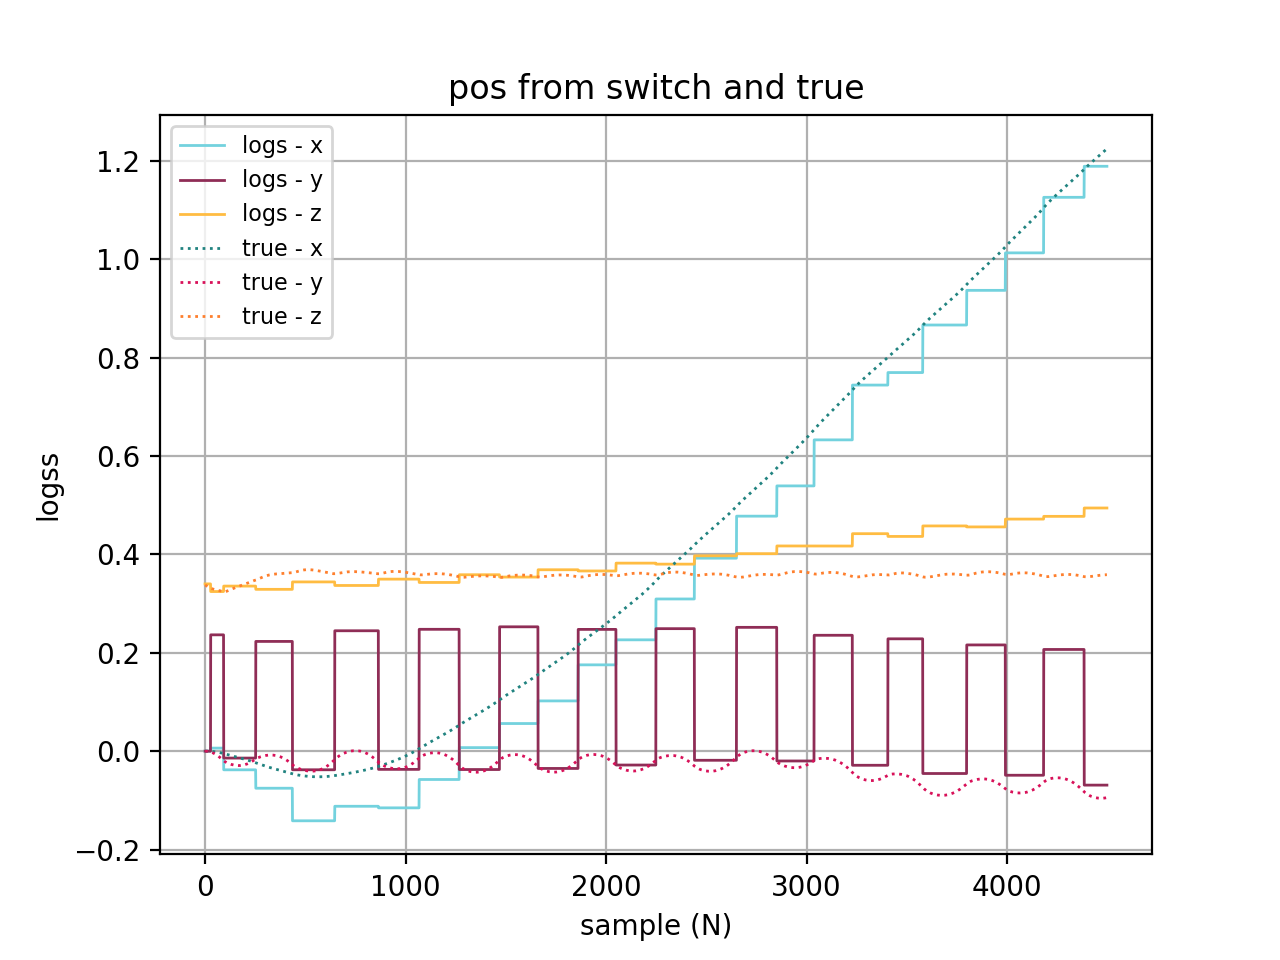
\includegraphics[width=\linewidth, angle=0, scale=0.7]{./images/switch_odometry.png}
  \caption{Switch odometry in Bolt simulation \mnaveau{Update title of the plot. true => ground truth + add label}}
\end{figure}

\subsection{Implementation}

The position $p_{out}$ is computed as follow : $\Delta p = p_{inter} - p_{switch}$ is computed every footstep. Then, during the following footstep, the error on $x$ is compensated by adding $\frac{\Delta p}{\Delta T_{footstep}}$ to the $p$ estimate. This way, assuming the drift is slow enough and the next footstep is about the same duration as the previous one, the drift will be compensated at the time of the next switch. Since the drift using 
$$ p_{inter} = \int_t v_{out} \, \mathrm{d}t $$
takes more than one second to become significant, the $x$ position drift can be compensated using the switch odometry.
As for the $z$ drift on position, it is corrected using the encoders. The estimator computes the $z$ distance between the foot in contact and the base every timestep, and use it to correct this drift.

\begin{figure}[H]
\centering
  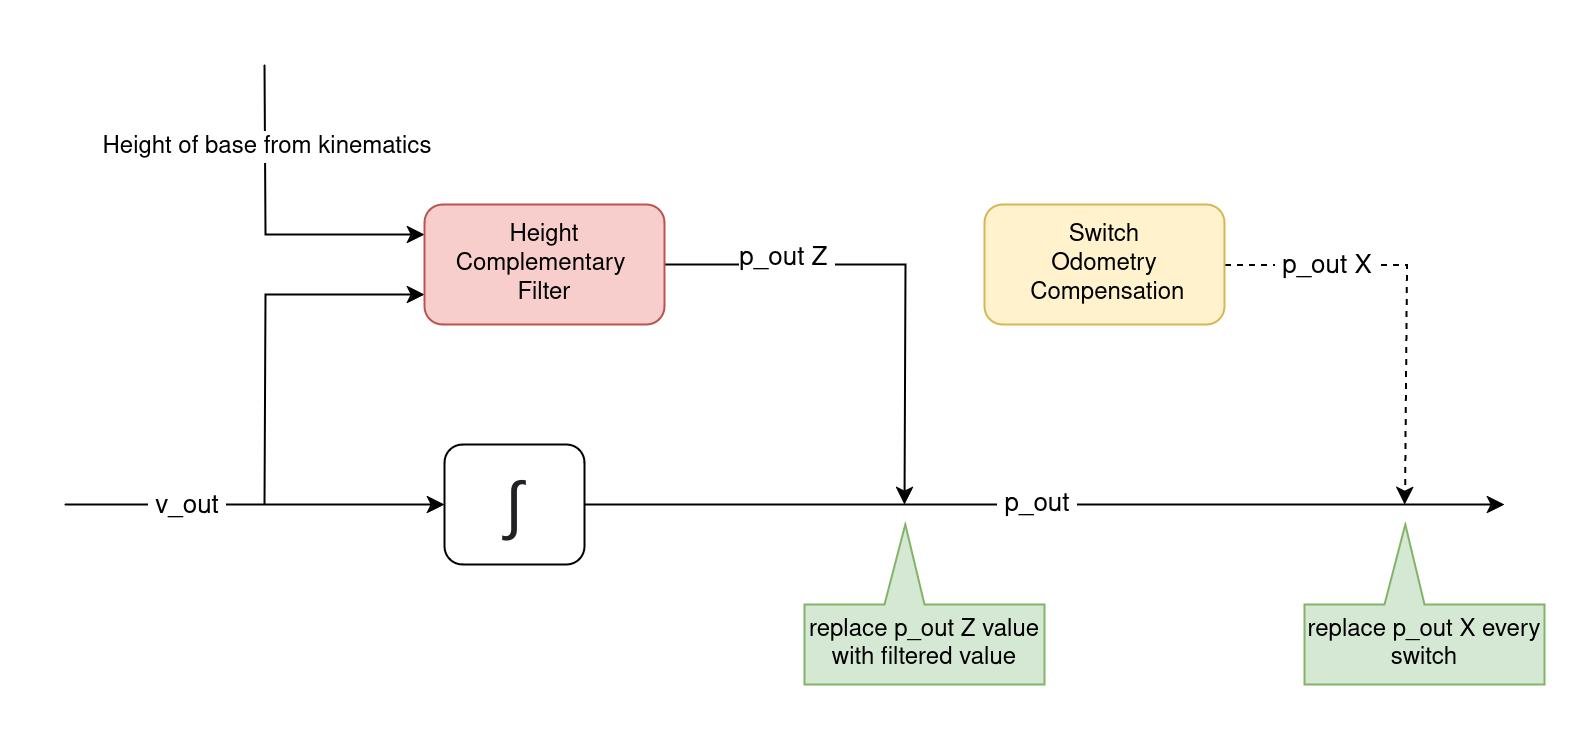
\includegraphics[width=\linewidth, angle=0, scale=1]{./images/Variable_Position.png}
  \caption{Position datapipe. \mnaveau{what is $pos\_outX$?}}
\end{figure}






\section{Testing}
\subsection{Testing Filters}
To test the filters, on can generate simple signals, add gaussian white noise to a certain intensity and feed it to the filter
Below is the structure in place for testing the different filters.
\begin{figure}[H]
\centering
  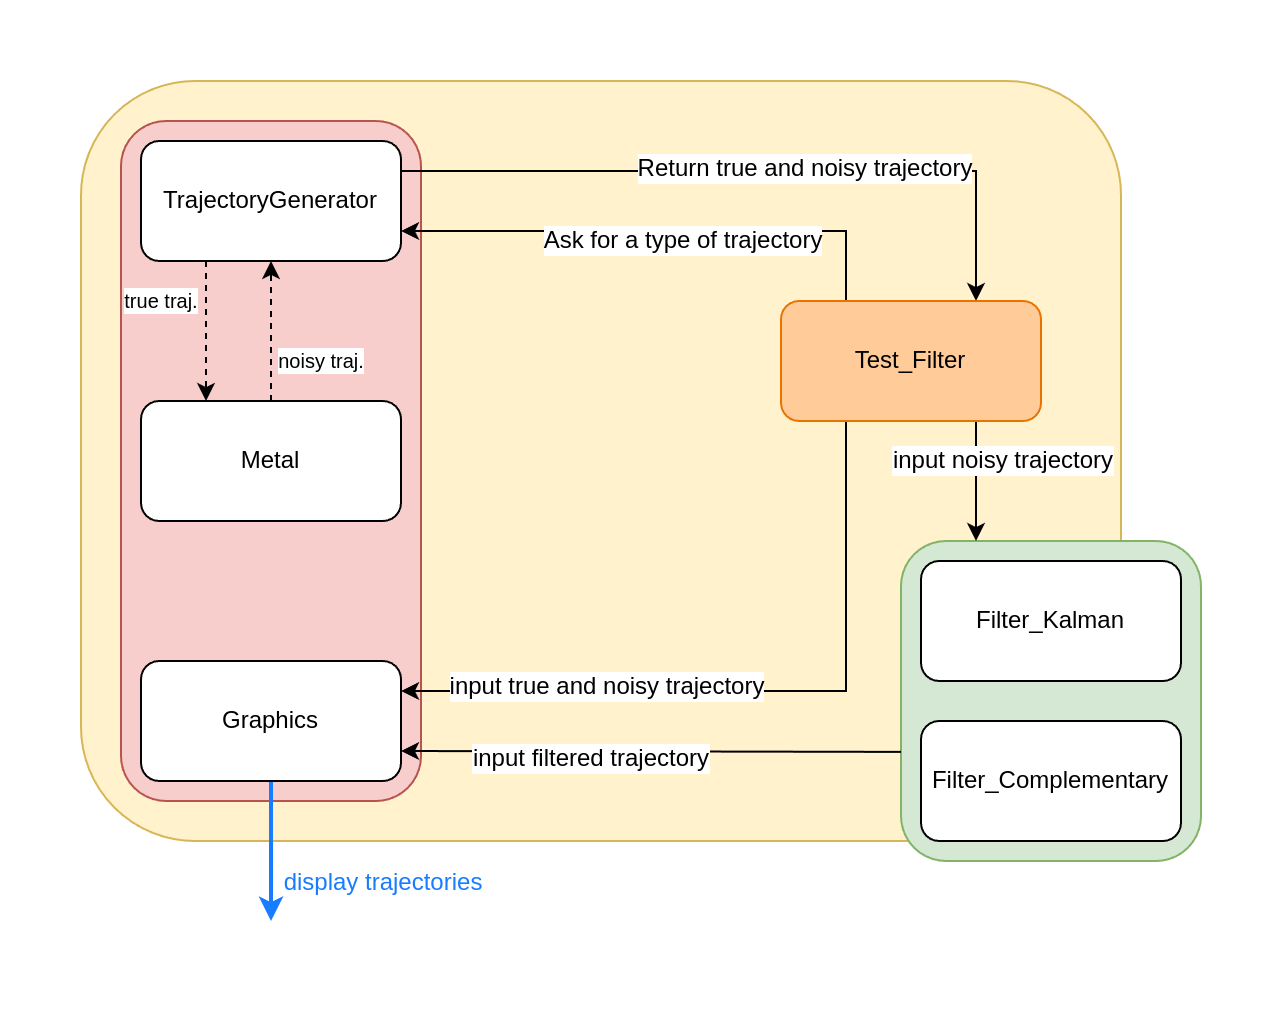
\includegraphics[width=\linewidth, angle=0, scale=1]{./images/Action_Test.png}
  \caption{Filter testing on simulation logs}
\end{figure}

\subsection{Testing Estimator on logs}
To test the main estimator and its sub-estimators, one can save logs from a simulation, and then run the estimator on this dataset. This allow to log the full state of the robot, including data that the estimator is not able to read (such as the base position, or the exact movement of the hip). This data can then be used to compare the estimator output to the simulated truth, and to understand what is going on during estimation.

Below is the structure in place for testing the Estimator on dataset extracted from simulation. DeviceEmulator acts as replacement for the ODRI interface, by providing data with the right names.
\begin{figure}[H]
\centering
  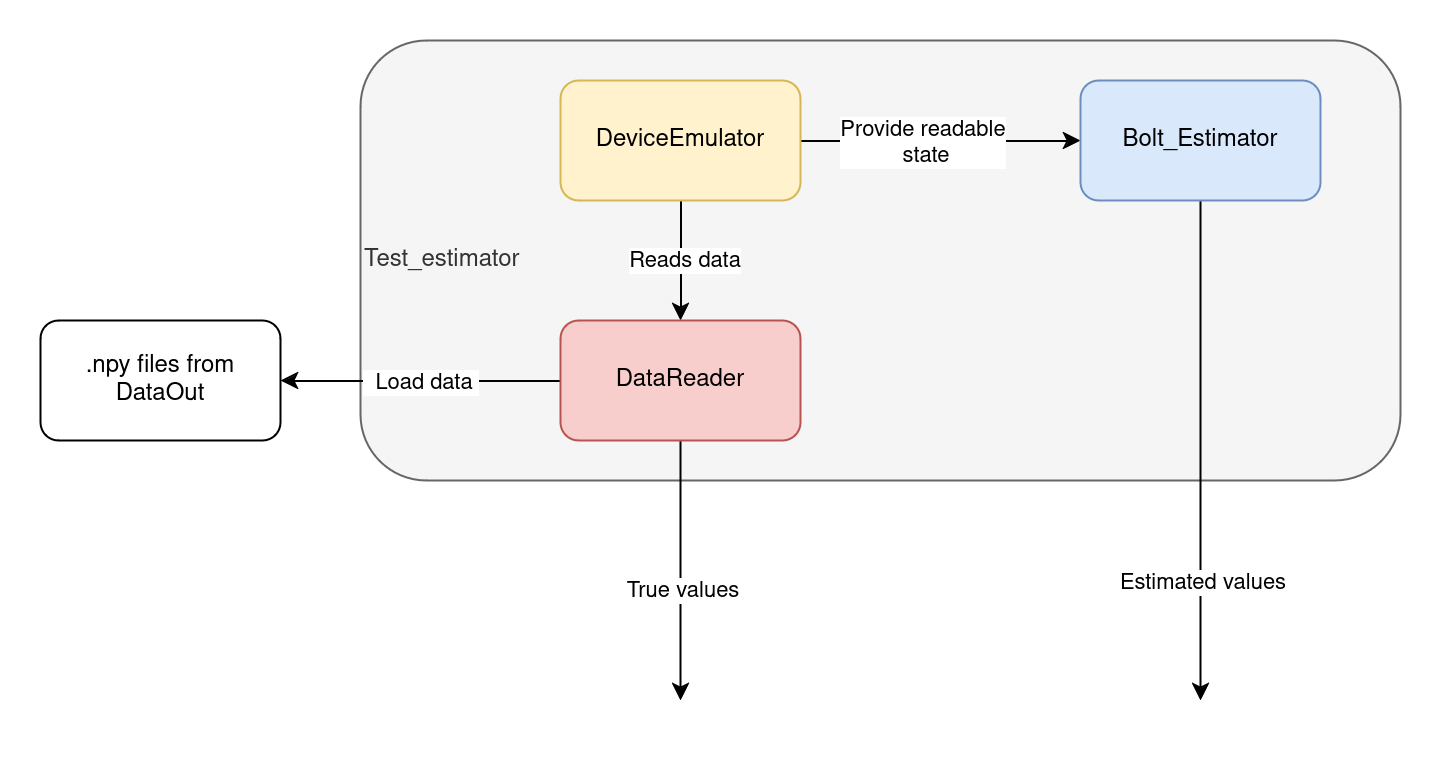
\includegraphics[width=\linewidth, angle=0, scale=1]{./images/Testing_estimator.png}
  \caption{Estimator testing on logs}
\end{figure}

I chose to test the estimator on four different datasets, with different $dt$ at $1$ms ($1$kHz), $5$ms ($200$Hz) and $10$ms ($100$Hz). Below are representative results obtained after a run of $3$s at $1$ kHz.

\begin{figure}[H]
\centering
  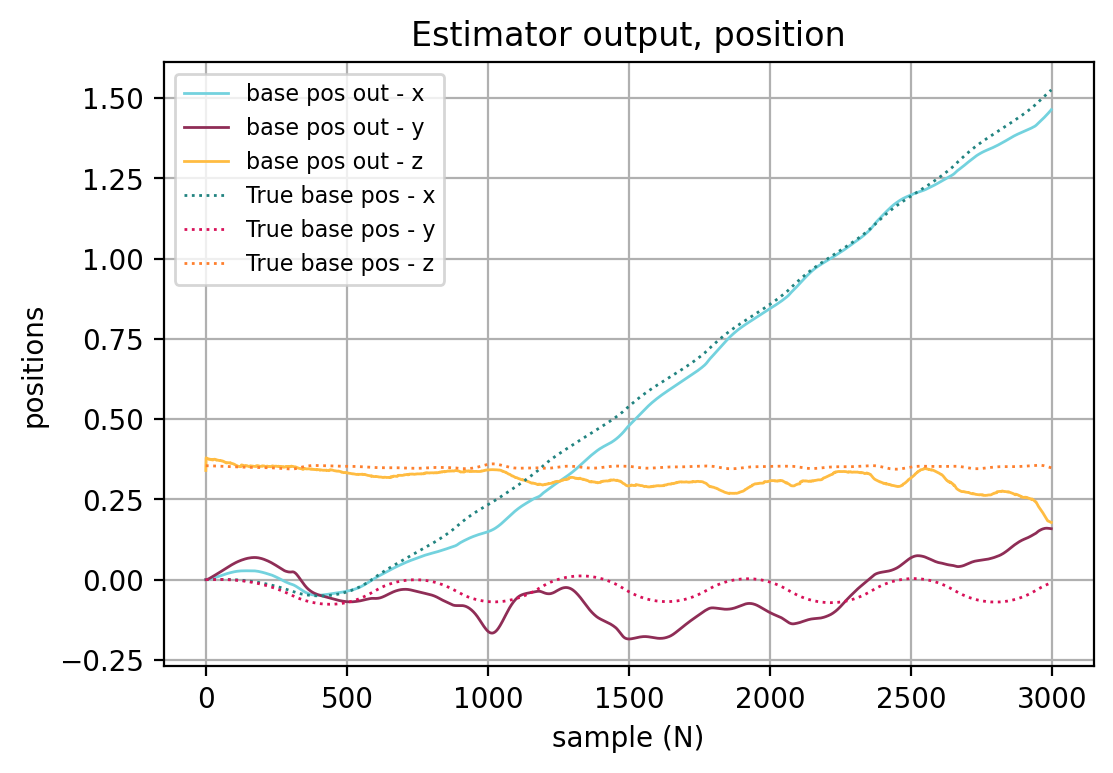
\includegraphics[width=\linewidth, angle=0, scale=0.8]{./images/resultat_simu_position.png}
  \caption{Position (with switch compensation starting at 1500ms)}
\end{figure}


\begin{figure}[H]
\centering
  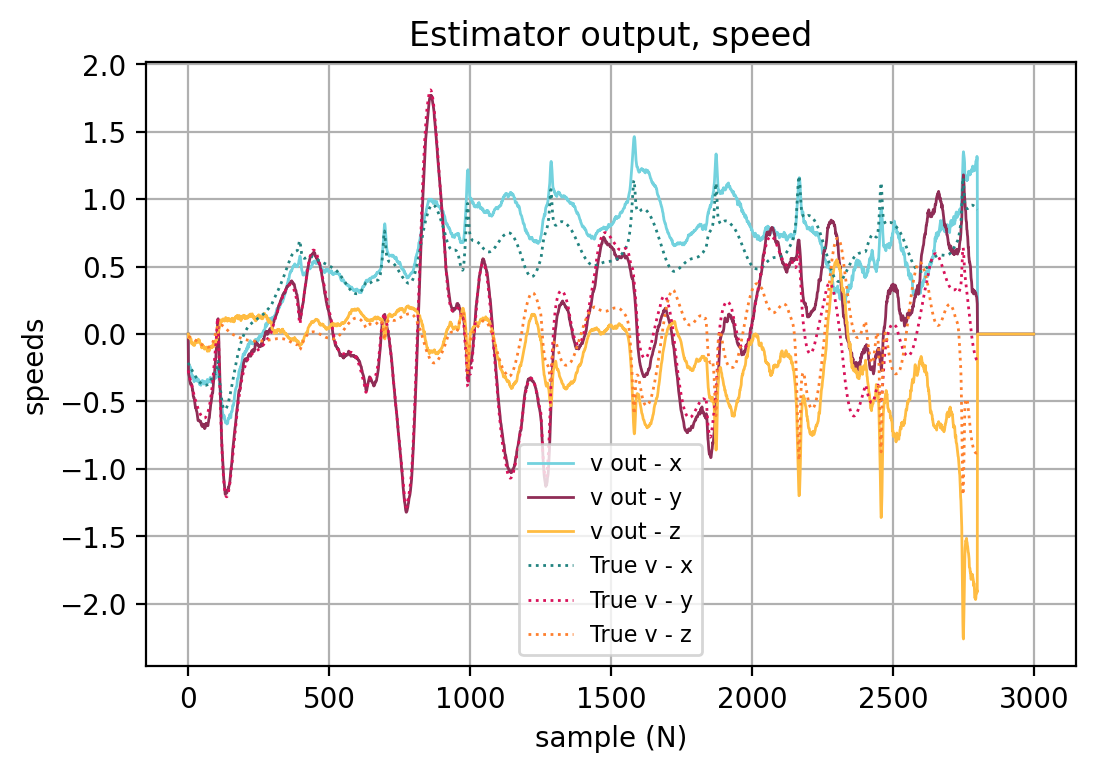
\includegraphics[width=\linewidth, angle=0, scale=0.8]{./images/resultat_simu_speed.png}
  \caption{Speed}
\end{figure}

\begin{figure}[H]
\centering
  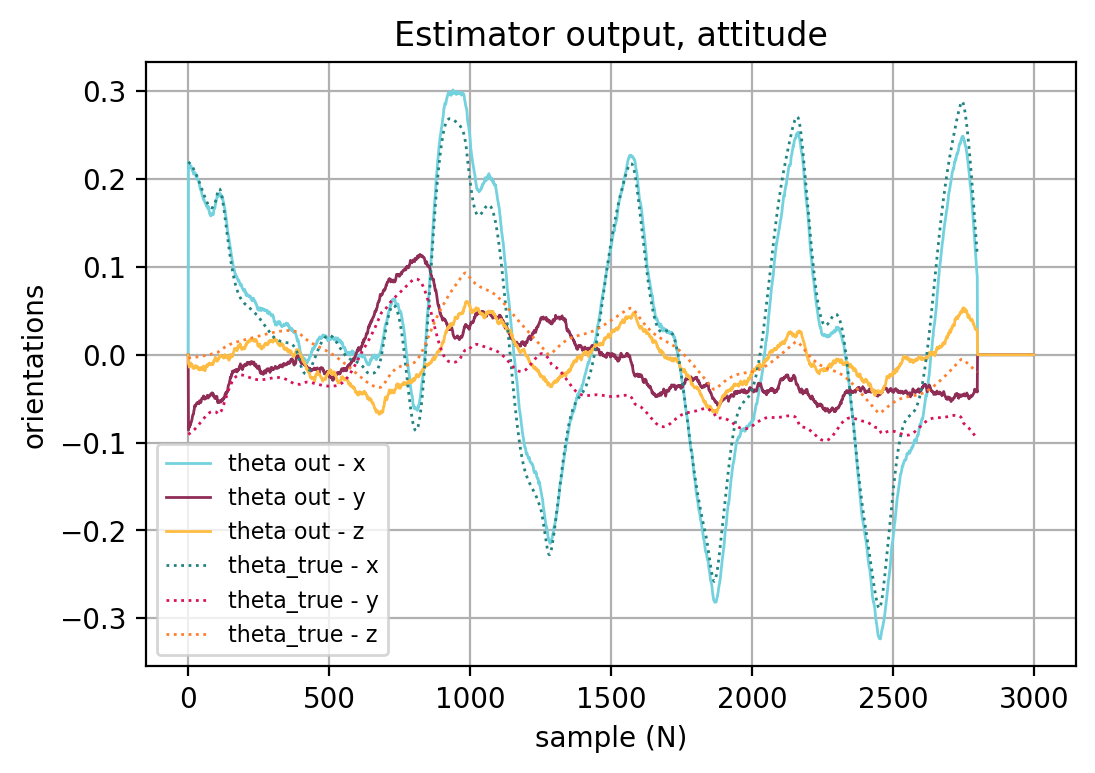
\includegraphics[width=\linewidth, angle=0, scale=0.8]{./images/resultat_simu_attitude.png}
  \caption{Attitude}
\end{figure}





\subsection{Testing Estimator in live simulation}
To further test the estimator, one can run it directly within the simulation. The estimator can be fed with true data from the solver. The estimated data it returns can be logged or used to compute the command. The true, command and estimated values can be plotted using DataLogReader.
\mnaveau{Un peu maladroit, je suis pas sur de comprendre...}


\section{Testing on Bolt}
As of August 2024, Bolt cannot walk stably by itself for a sufficient amount of time to test the estimator precisely. Yet, the estimator was runned on Bolt in real life. The setup of the experiment was as follow : 
\begin{itemize}[noitemsep,topsep=0.5pt,parsep=0.1pt,partopsep=0.1pt]
  \item Bolt was plugged to a external $24$V alimentation
  \item Bolt was wired to a laptop with high computing power, running a downgraded code from C.Roux \cite{15} (an unreleased version of his MPC \cite{1}) alongside the estimator.
  \item Bolt was preventing from falling by a string
\end{itemize}
This led to Bolt executing a few estimated footsteps before fall. The code ran at around $450$Hz to $550$ Hz. It is to be noticed that the estimator alone runned at over $2$kHz on the same computer, and the command part at around $1$kHz. This emphasize that this first experiment was probably not computationnaly efficient enough.

\subsection{Testing with IMU and MoCap}
Tests were conducted using simultaneously Bolt's internal sensors and MoCap. Bolt's command was disabled by setting it to zero at all time. The read values of IMU could then be compared with values from MoCap and Estimator. Yet, IMU provides data relative to acceleration and speed (eg $\dot x$ or $\ddot x$), while the MoCap provides very accurate $x$ measurements and a very poor first-order time derivative measurements ($\dot x$). This is because a $1$mm error in a $300$Hz measurement by MoCap is typical, and a pretty good estimate of $x$. But it gives us an error of $0.3$ m/s in speed, which is catastrophic for Bolt whose walking speed is around $0.2$ m/s.\\
Even if MoCap data can be filtered, using for instance a complementary filter with Bolt's onboard IMU, it proved difficult to compare MoCap, IMU and Estimator results, given that all were very unreliable. The few observations I made were that:
\begin{itemize}
 \item Tilt estimate from IMU was great as long for long period of time ($>10$s) as Bolt remained stable.
 \item Tilt estimate from estimator was noisier than IMU's while the robot was still, but better when the robot was moving. $theta_{tilt}$ proved more accurate than $theta_{out}$, which means that tuning has to be adapted between simulation and reality, the gaits being different.
 \item Speed estimate from Estimator seemed reasonnably accurate.
 \item Position estimate from Estimator was drifting after a few seconds. The chaotic gait of Bolt at that time probably did not help, as it was harder for the estimator to get contact information.
 \item peak happened on every data whenever a choc appeared, which was to be expected, but post-filtering data were still disturbed by it much more than in simulation.
\end{itemize}
Even if these experiments did not allow a serious benchmarking, they showed that the Estimator can be run on the real robot, and that it provides non-absurd results. It also highlighted the quality of the IMU, and the critical importance of handling shocks properly. It is to be mentionned that on Solo's code (see \ref{explanation_solo}) measurement are disabled around the time of the switch.


\section{Hardware modification}
\subsection{Goals}
Bolt is an open-source project, meaning that all plans and information on hardware and software are freely available. This allows one to easily modify or re-design some parts of the robot.
\st{I had to do this for several reasons.}
The next paragraph describes the changes made that was needed upon testing the estimator on-board of the robot.


\subsection{Wiring}
As Bolt had been damaged and dismanteled during previous experiments, we put the boards back in place and re-wired the robot with C.Roux, following instruction on \cite{2}.

\subsection{Stand}
A stand was made previously for Bolt. However, it was ill-suited for the robot, as Bolt was unstable when on it. Plus, its legs were touching the ground. I redesigned a new one, partly inspired by the photograph of Bolt stand available on \cite{2}. However, I changed the dimensions and added several parts to it. The stand is made out of 4 aluminum profiles, 4 brackets, and 3 \mnaveau{(3 parts? the picture only shows 2...)} 3D-printed parts.

\begin{figure}[H]
\centering
  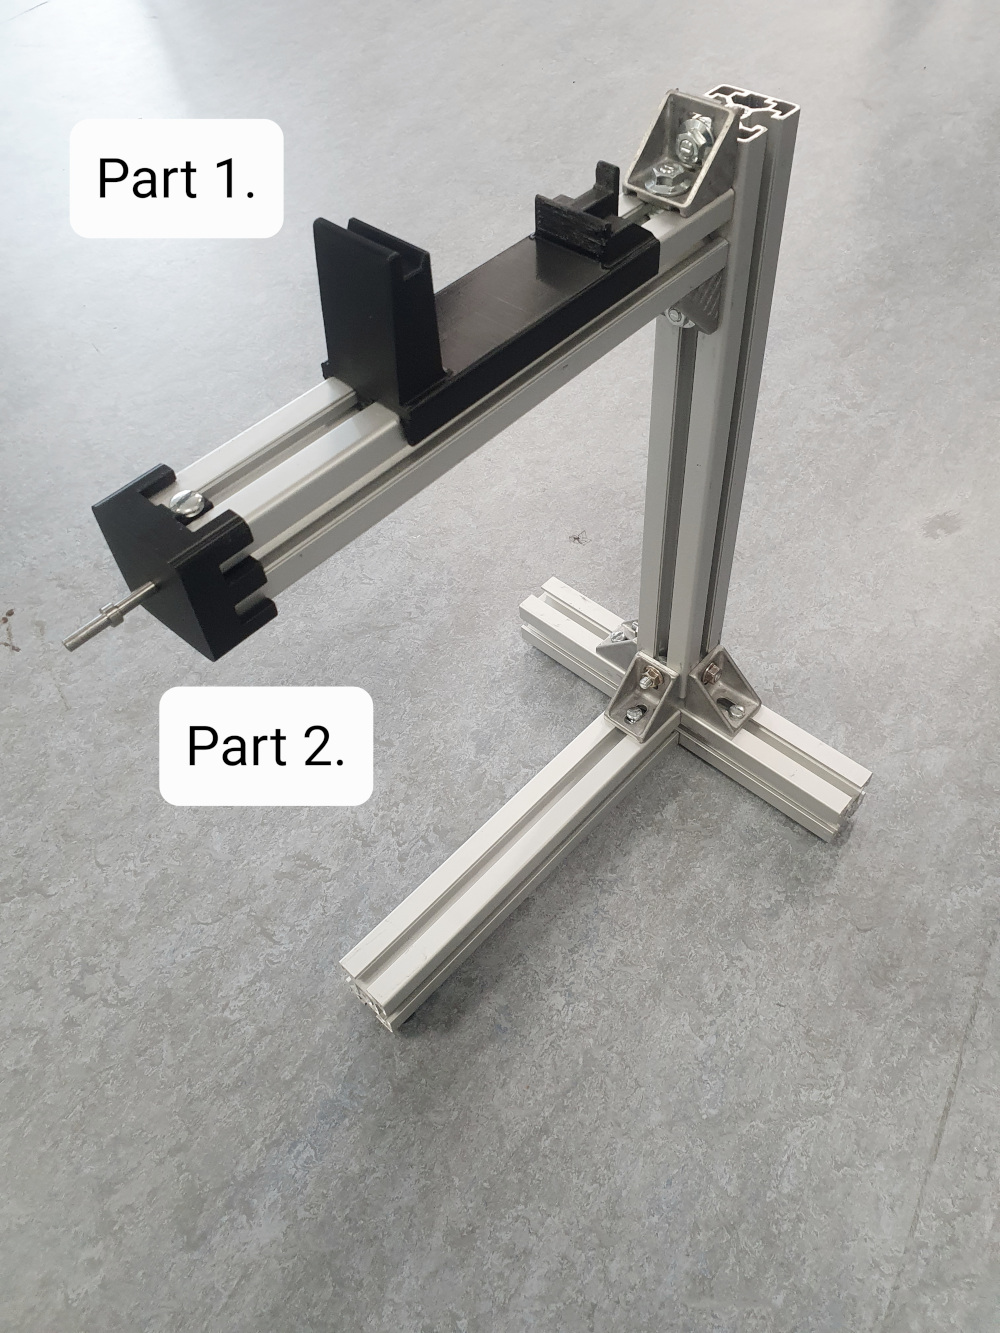
\includegraphics[width=\linewidth, angle=0, scale=0.4]{./images/Bolt_stand_0.jpg}
  \caption{The new Bolt stand}
  \label{Bolt's stand}
\end{figure}

Bolt can be placed either on top of the horizontal bar as in \ref{Bolt in position 1} or on the protruding axe. In the first case, its feet cannot touch the ground and its legs can move freely. The body is firmly held due to the V-shape of the front and back parts of Part 1. Part 1 can slide back and forth. This position is useful for calibrating the robot.



\begin{figure}[H]
\centering

\begin{subfigure}{.5\textwidth}
\centering
  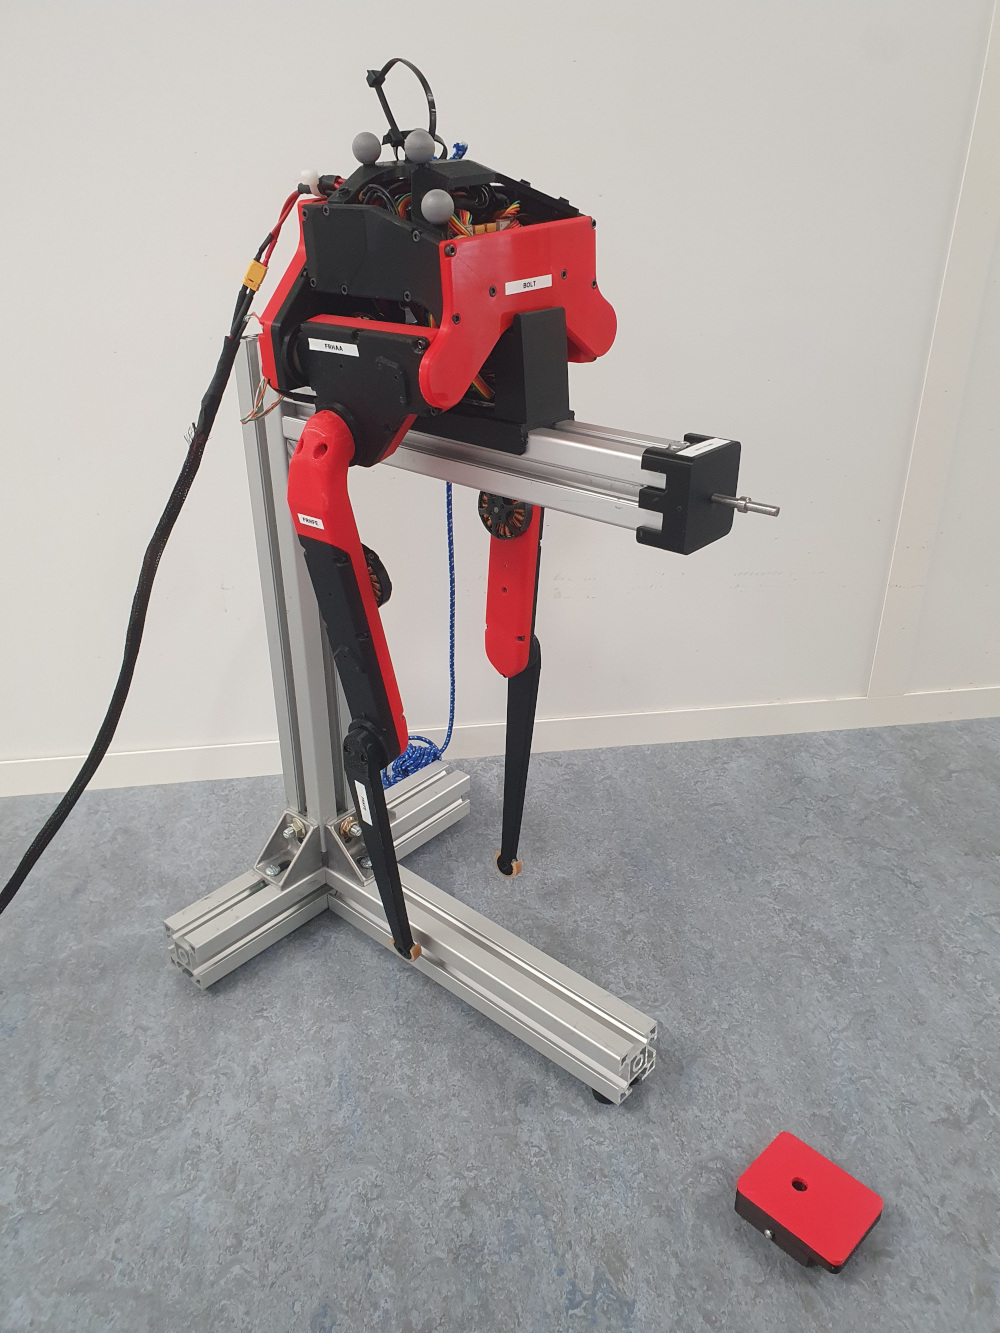
\includegraphics[width=1\linewidth, angle=0, scale=0.8]{./images/Bolt_stand_1.jpg}
\end{subfigure}%
\begin{subfigure}{.5\textwidth}
\centering
  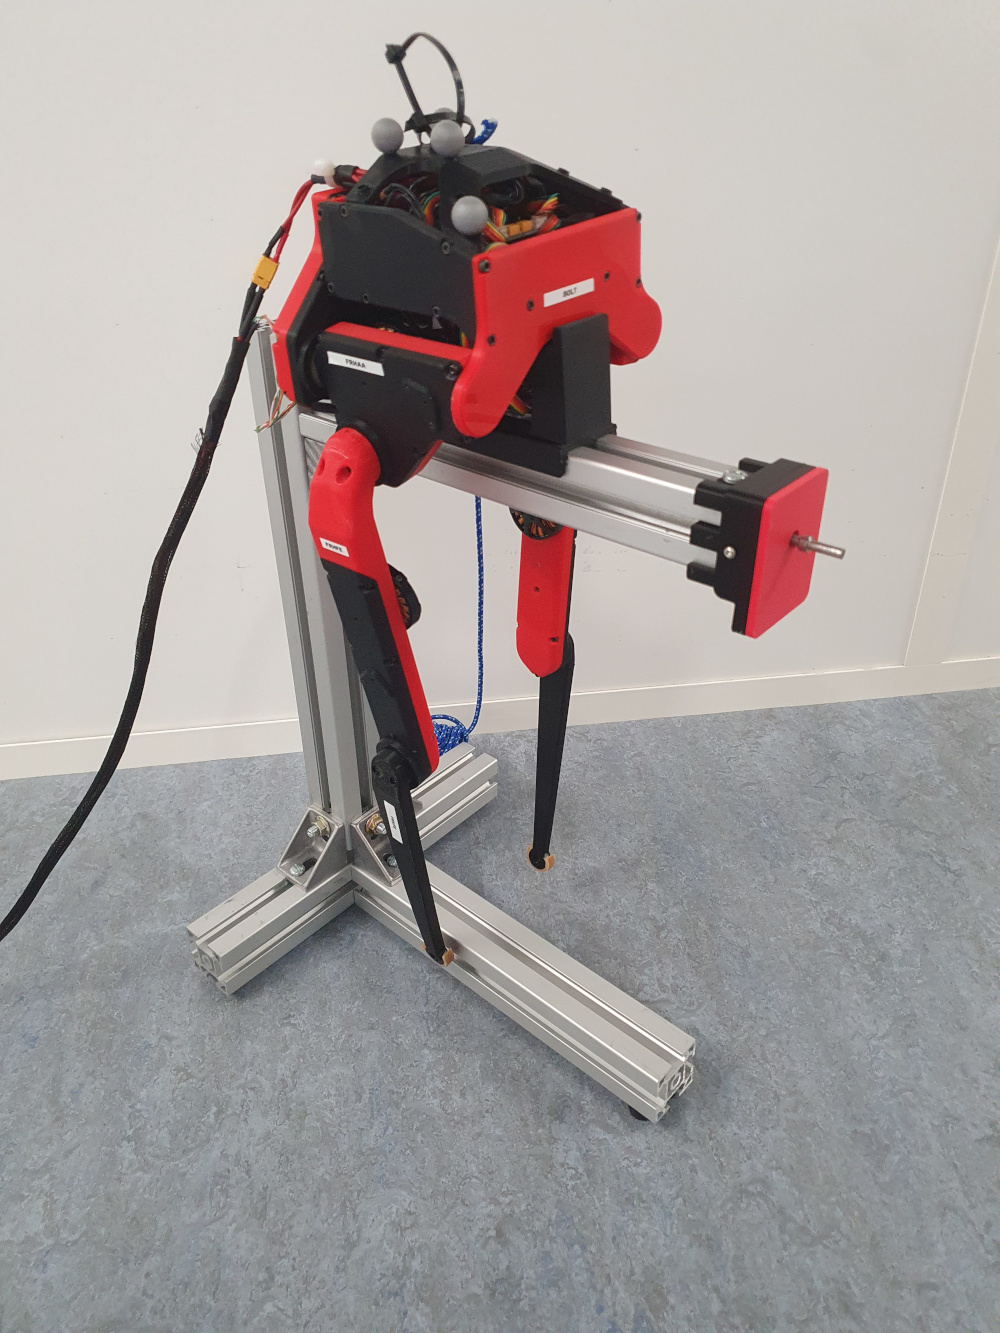
\includegraphics[width=1\linewidth, angle=0, scale=0.8]{./images/Bolt_stand_2.jpg}
\end{subfigure}
\caption{Bolt in position 1, with and without Part 3 on.}
\label{Bolt in position 1}
\end{figure}

When Bolt is placed on the protruding axis, its base height is such that it is in its ideal starting position. Part 3 can be put in front of Part 2, or not. If it is, the robot will be held only by the very end of the axis. Its back leans against Part 3, ensuring it is in a vertical position and not leaning forward. This allows the robot to be in a good starting position for a walk, and detach itself from the stand at the very start of its movement. If Part 3 is not on, the robot will lean slightly forward, but will have a firmer attach to the stand, preventing it from falling easily.\\

\vspace{5mm}

The axis used is 5mm in diameter and around 56mm in length. Part 2 has a central extension inside the aluminium profile, to hold the axis strongly. The axis can be screwed to the back of Part 2. I recommend Part 2 to be printed with reasonnable quality and high strength settings, with an infill of around 35\%. Dimensions of parts 2 and 3 were made for a specific aluminium profile, as their shapes closely match those of the profile. All parts were printed in PLA.

\begin{figure}[H]
\centering
  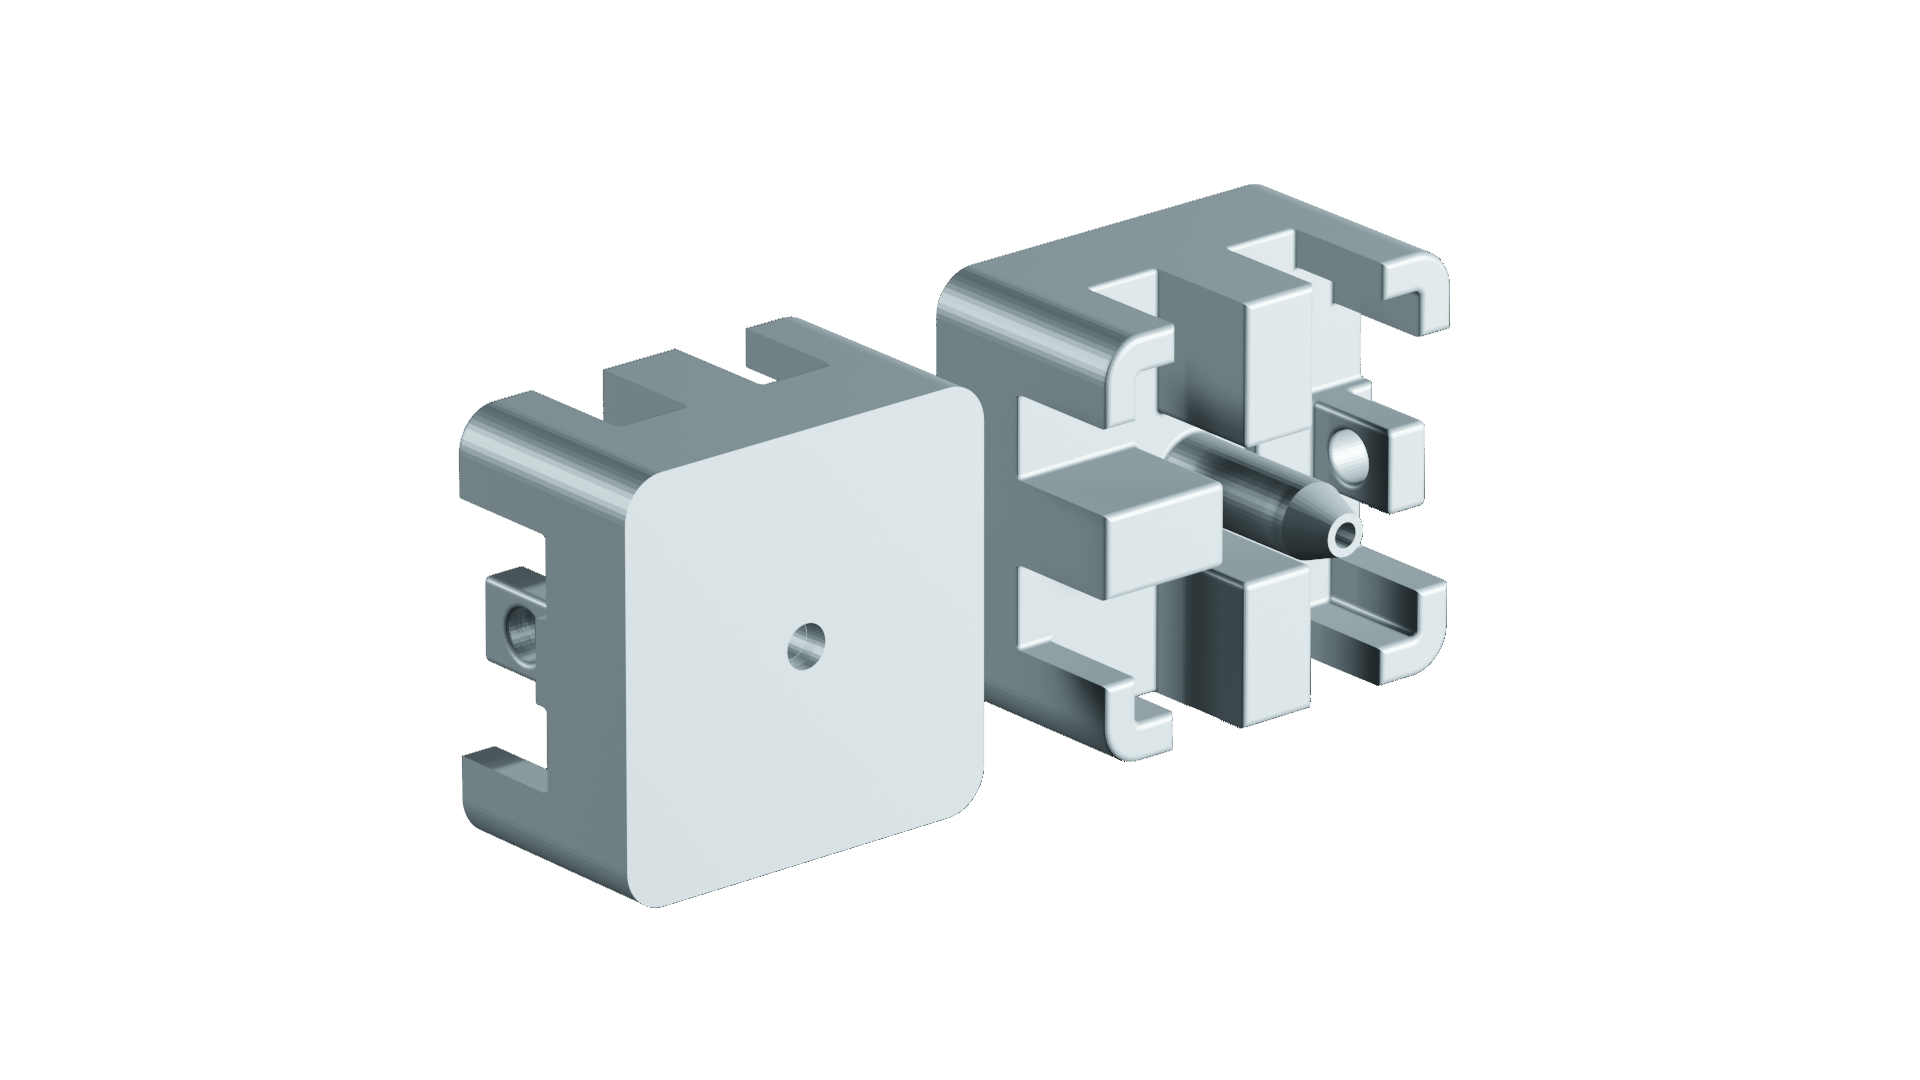
\includegraphics[width=\linewidth, angle=0, scale=0.8]{./images/render_stand.png}
  \caption{render of Part 2}
\end{figure}




\subsection{Bolt's hat}
The hat that was originally printed for Bolt has many supports for MoCap markers, but all are very close from one another. This proved to cause issues with the MoCap system at LAAS, probably because the marker used were bigger than those originally fitted. Additionnaly, the hat was not very strong. I designed and built a new hat, which features more dissymetric and distant MoCap markers mounting points, a stronger build, and a hook. The hook can be used to attach a cable to lift the robot, or hold it in the event of a fall. Due to the additionnal thickness, the hat protrudes upward slightly from Bolt's chassis. It took three iterations of this part to get the MoCap markers placement right.

\mnaveau{It would be nice if you get the previous hat picture and model in picture here to see the differences.}

\begin{figure}[H]
\centering

\begin{subfigure}{.5\textwidth}
\centering
  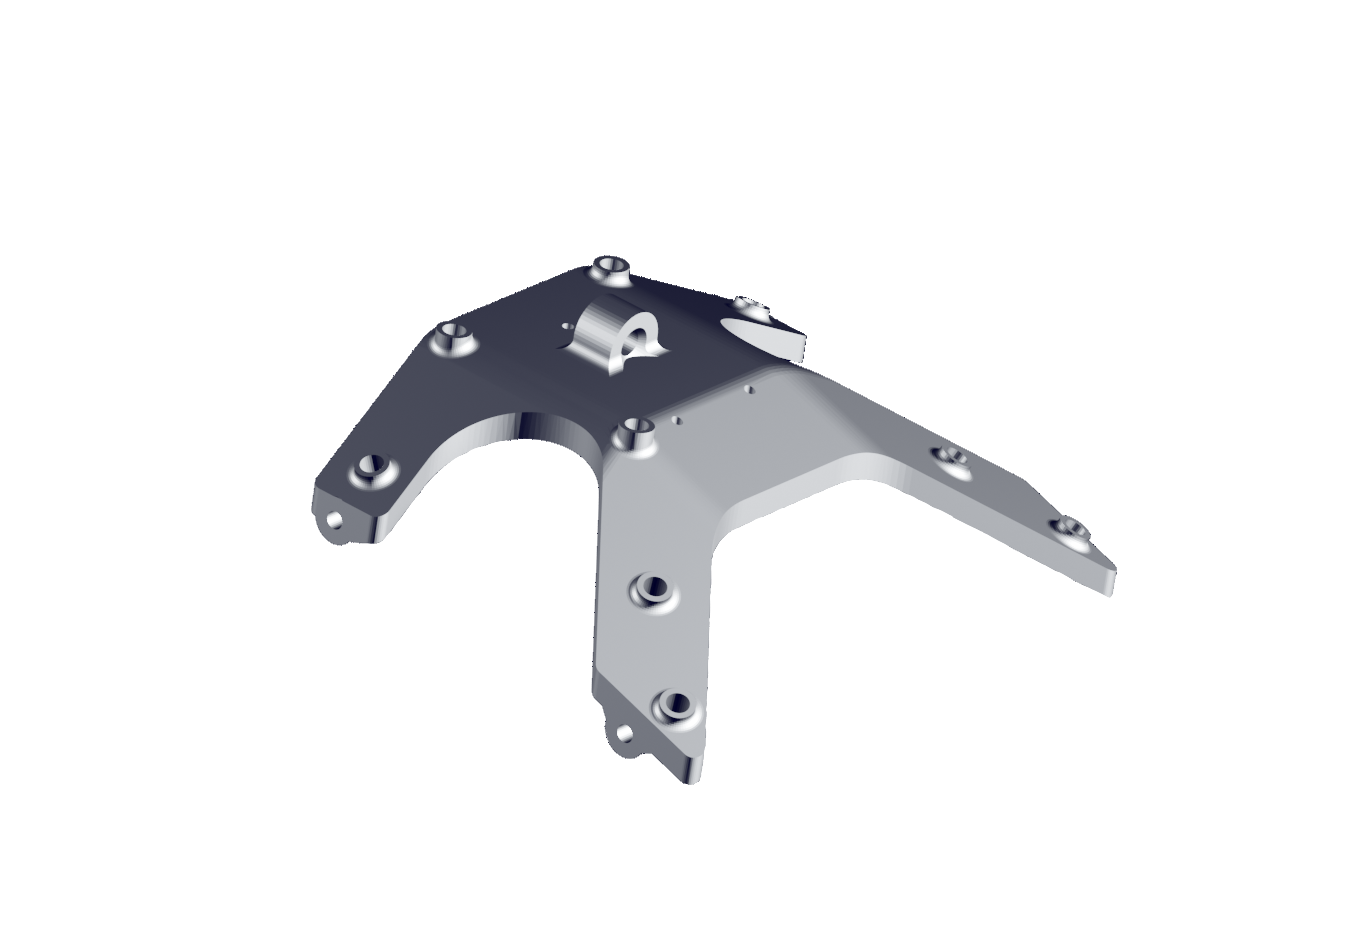
\includegraphics[width=1\linewidth, angle=0, scale=1.2]{./images/render_top.png}
  \caption{Render of the new hat}
\end{subfigure}%
\begin{subfigure}{.5\textwidth}
\centering
  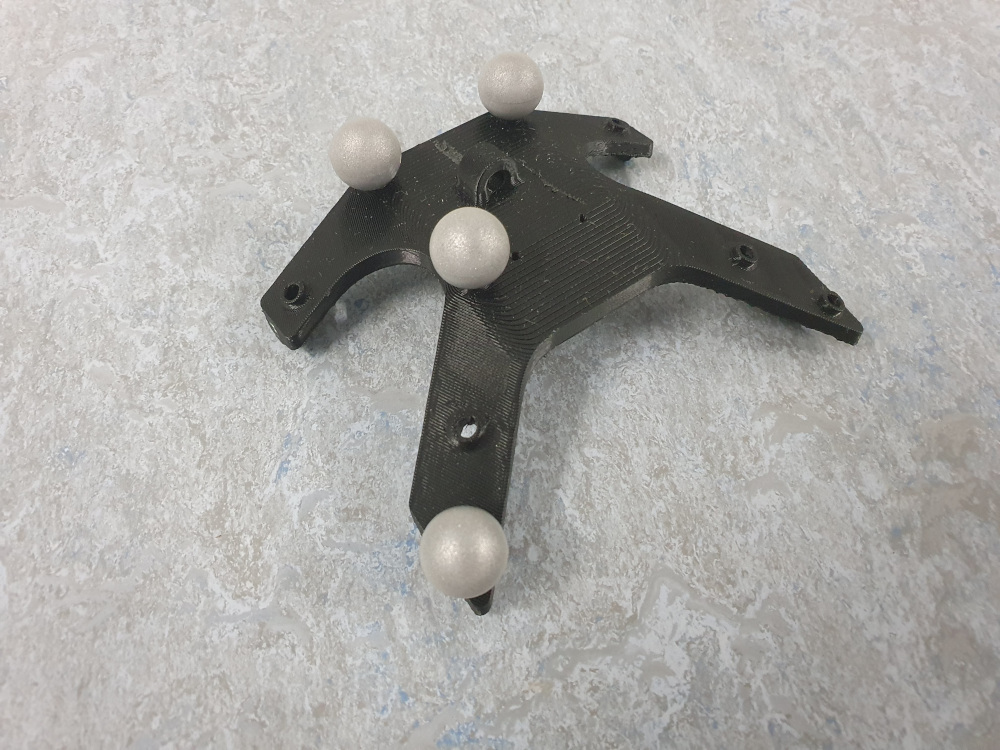
\includegraphics[width=\linewidth, angle=0, scale=0.9]{./images/Bolt_hat.jpg}
  \caption{The new Bolt hat and the MoCap markers we used}
\end{subfigure}
\caption{Bolt's new hat}
\label{Bolt new leg}
\end{figure}



\begin{figure}[H]
\centering
  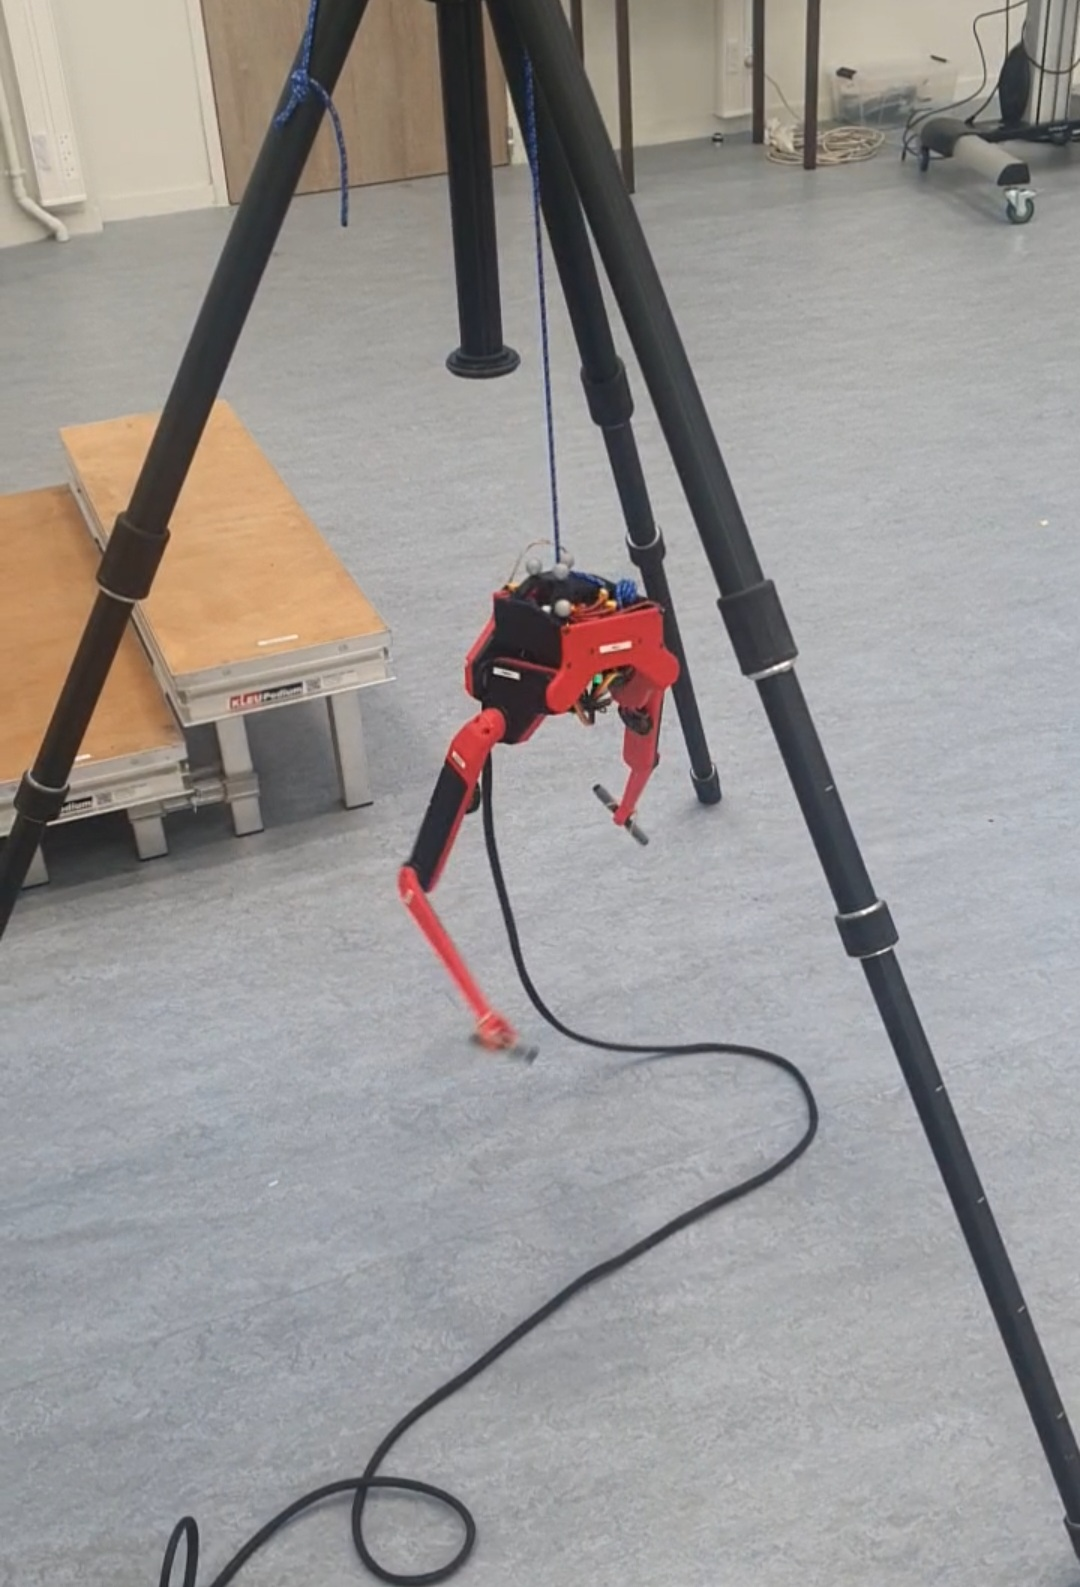
\includegraphics[width=\linewidth, angle=0, scale=0.3]{./images/Bolt_testing.jpg}
  \caption{Hooking Bolt for testing}
  \label{New Bolt hat}
\end{figure}



\subsection{Bolt's legs}
Bolt's original legs have a distinctive passive actuator on the ankle, and a cylindric foot. To get closer to the URDF design and for testing purpose, I designed a new leg, with the same length and shape as the URDF's leg. In both case, the foot-ground contact is more or less a sphere-plane contact.

\mnaveau{For the story, in max planck we firstly designed a leg like the one you drawn. And then we decided to go with linear contact because the control was made a bit easier this way. So it's not really "new". Please check the ODRI github in Bolt if you cannot find the old legs from Felix Grimminger.}

\begin{figure}[H]
\centering

\begin{subfigure}{.5\textwidth}
\centering
  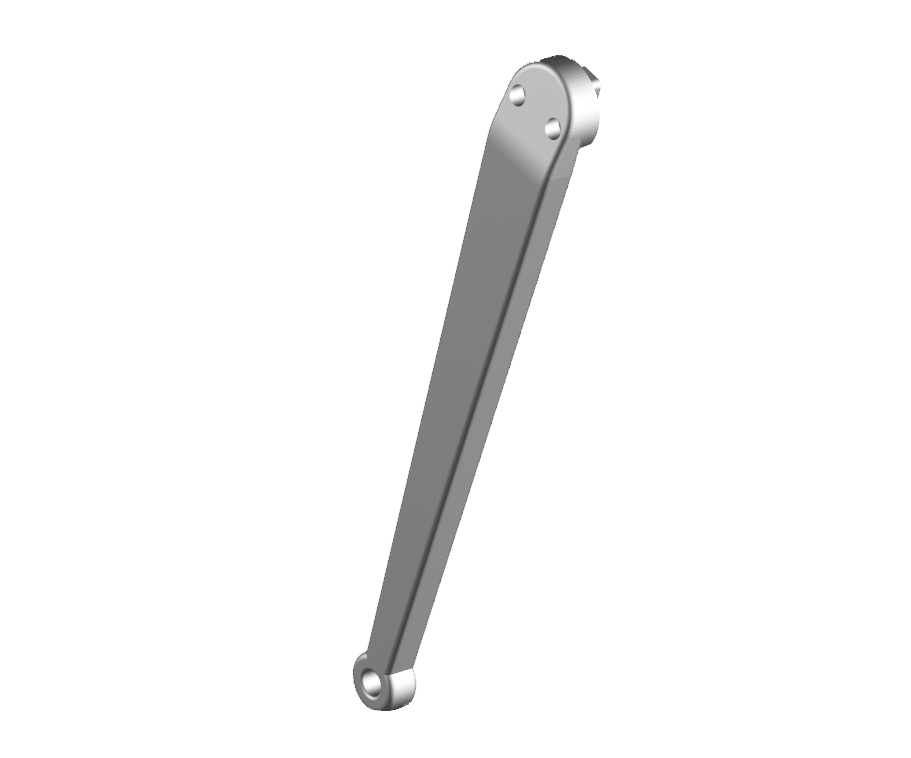
\includegraphics[width=1\linewidth, angle=0, scale=1.2]{./images/render_leg.png}
  \caption{Render of the new leg}
\end{subfigure}%
\begin{subfigure}{.5\textwidth}
\centering
  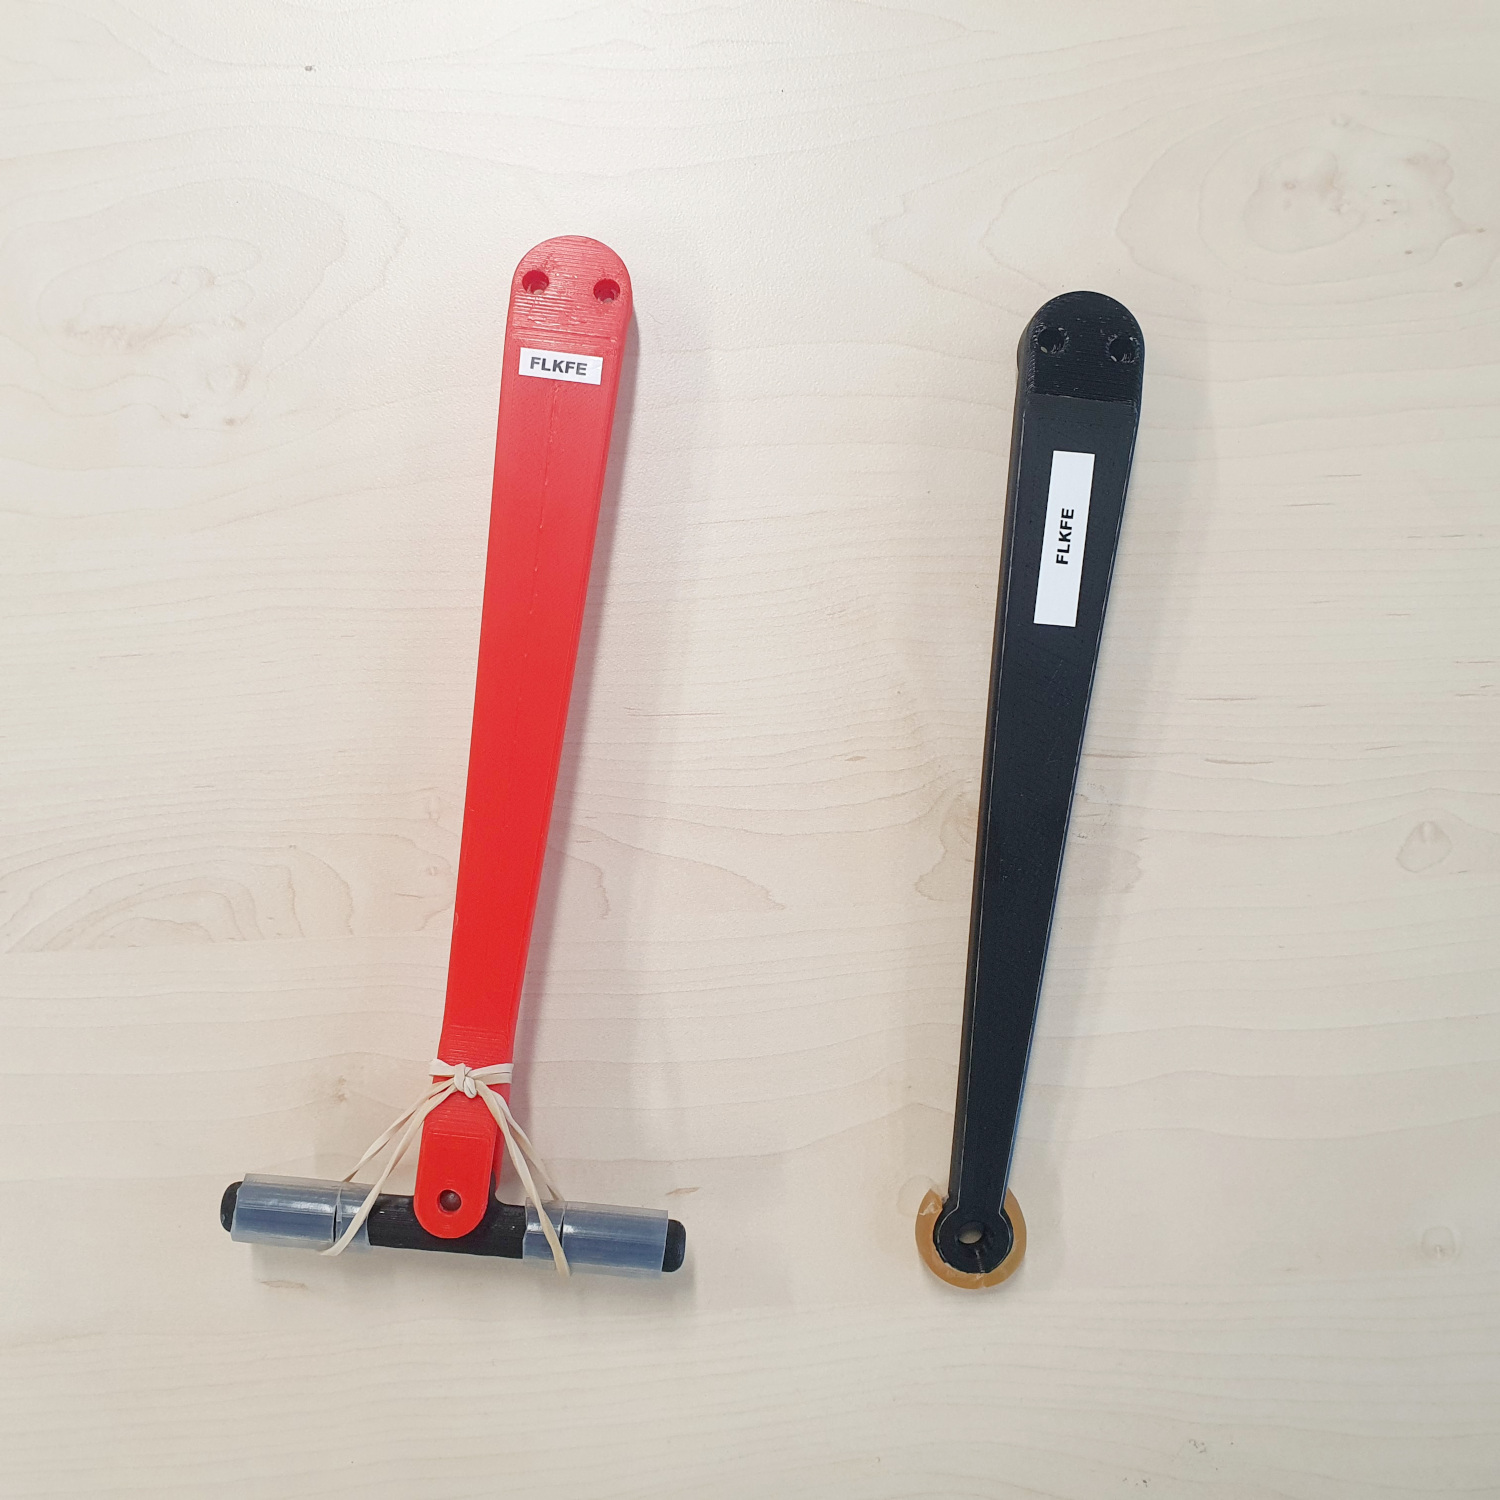
\includegraphics[width=\linewidth, angle=0, scale=0.9]{./images/Bolt_leg.jpg}
  \caption{Leg with passive actuation in red, new leg with rounded end in black}
\end{subfigure}
\caption{Bolt's new leg}
\label{Bolt new leg}
\end{figure}










\section{Context}
\label{context}
This section formally introduces the organizations mentionned in this document.

\subsection{What is CNRS ?}
CNRS is the french abbreviation for National Scientific Research Center. CNRS is mainly funded by the French government, and has many compounds all over France. Founded in 1939, it is widely multidisciplinary and has strong international connections.\\
\url{https://www.cnrs.fr/en}


\subsection{What is LAAS ?}
LAAS is a research laboratory, part of CNRS. It focuses on computer science, robotics, automation, and nano-technologies. Located in Toulouse, S-W of France.\\
\url{https://www.laas.fr/en/}

\subsection{What is Gepetto ?}
Gepetto is a team of researchers, working at LAAS and specialized on legged robots.\\
\url{https://www.laas.fr/en/teams/gepetto/}


\section{Explanations}
\label{explanations}
This section will hopefully answers your questions over various aspects of this work. It defines several terms, as they are used in this document. They are not to be considered as formal definitions, but rather as a starting point for latter research if needs be. Moreover, the following notions are merely put in the context of this document. For more information, make use of the references linked to each of the following point.\\


\subsection{What is Bolt ?}
Bolt is a bipedal robot, around 40cm in height and 1.3kg heavy. It is an open-source project, whose CAD can be found here : \url{https://github.com/open-dynamic-robot-initiative/open_robot_actuator_hardware/blob/master/README.md}\\
It was developped under the Open Dynamics Robot Initiative. Bolt is the 2-legged version of Solo, which is 4-legged. Bolt has 6 DoF, 3 per leg. Its ankle are unactuated. 
\begin{figure}[H]
\centering
  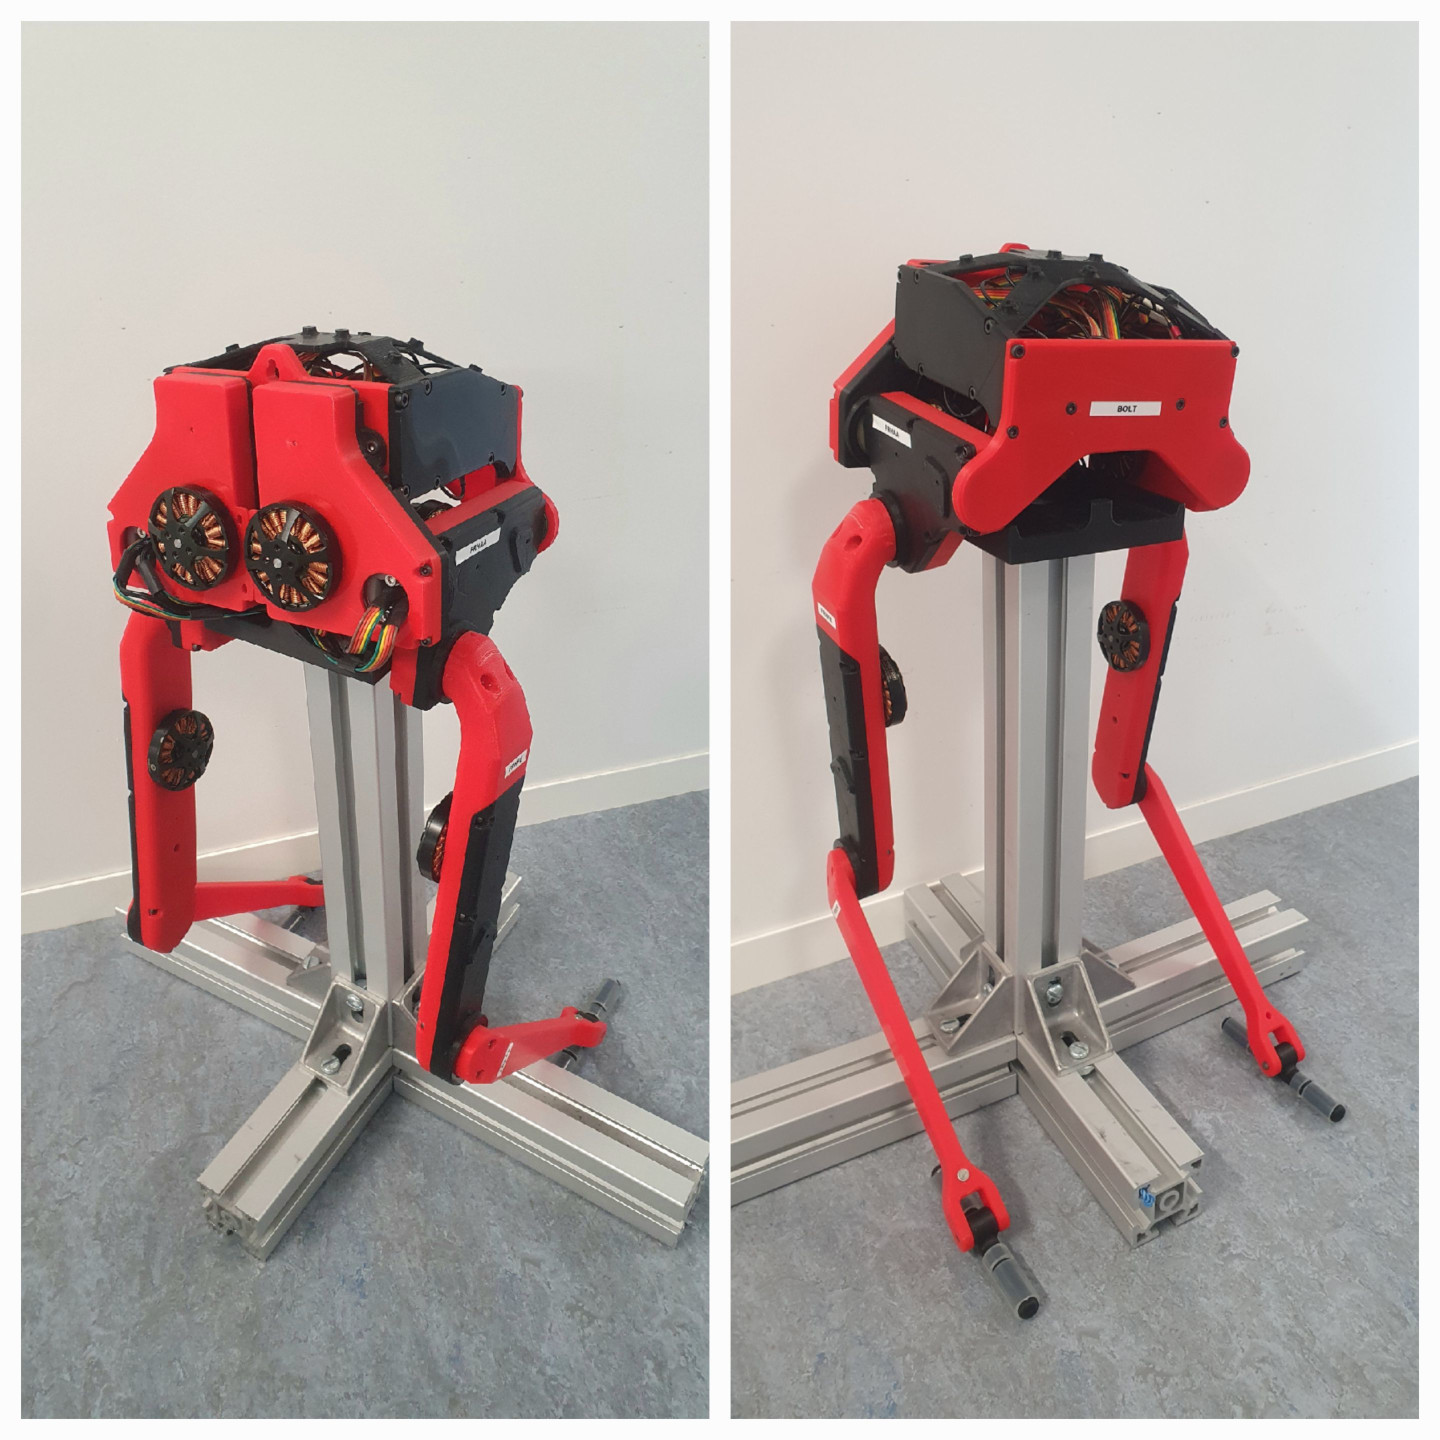
\includegraphics[width=\linewidth, angle=0, scale=0.5]{./images/Bolt0.jpg}
  \caption{Bolt}
\end{figure}

\subsection{What is Bolt's base ?}
Bolt's base is what would be its pelvis, should Bolt have been human. In fact, given the physionomy of Bolt, it is anything but its legs.

\subsection{What is an IMU ?}
IMU stands for Inertial Measurement Unit. It is a set of sensors, including at least a 3D accelerometer and a 3D gyroscope, which gives us a 6-axis IMU, that can be extended with a magnetometer, which gives us a 9-axis IMU. 
\begin{figure}[h]
\centering
  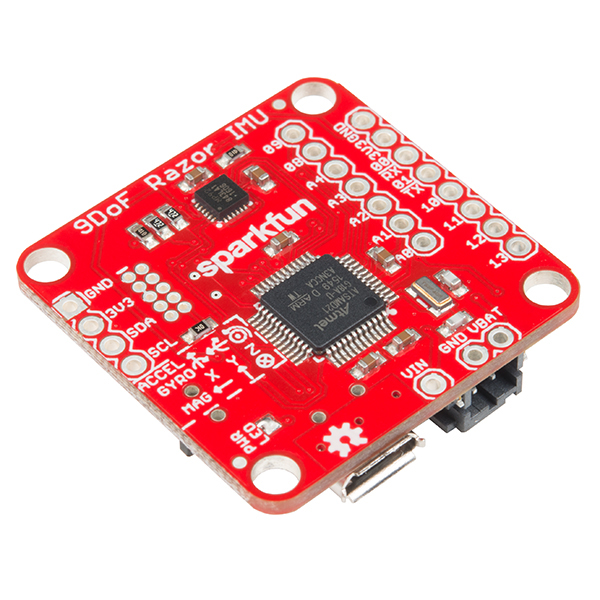
\includegraphics[width=\linewidth, angle=0, scale=0.2]{./images/IMU.jpg}
  \caption{IMU}
\end{figure}

\subsection{What is MoCap ?}
MoCap is the abbreviation for Motion Capture, and refers to a system of $n$ cameras being used to derive the position, attitude, speed, etc of a given object in space. For the cameras to understand where the object is, specific markers are added on known spots on the object.
\begin{figure}[h]
\centering
  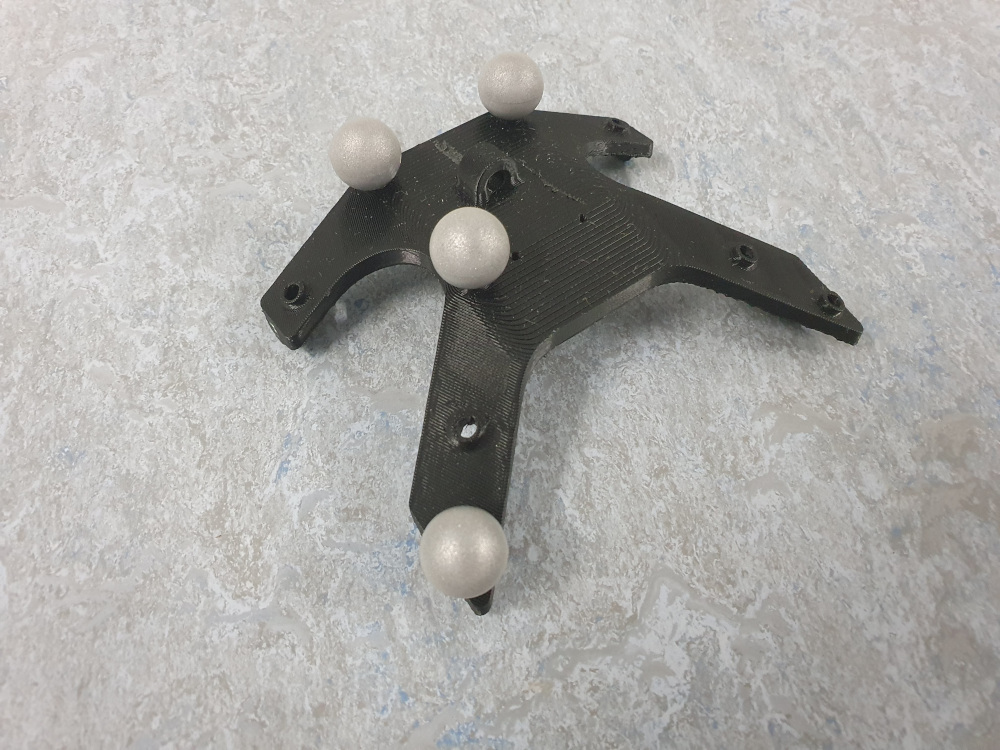
\includegraphics[width=\linewidth, angle=0, scale=0.2]{./images/Bolt_hat.jpg}
  \caption{Bolt's new hat with 4 MoCap markers}
\end{figure}

\subsection{What is a DoF ?}
DoF stands for degree of freedom. It is the number of parameter you can independantly change in a system. A leg with $k \in \mathbb{N}$ DoF has $k$ controled joints that can be controled independantly.


\subsection{What is Attitude ? What is Tilt ?}
The attitude, or tilt, is the set of three angles our robot makes with a world reference. The robot might tilt left (roll), tilt nose-down (pitch), or circle around on the floor (yaw).\\
 \url{https://en.wikipedia.org/wiki/Orientation_(geometry)}
 

\subsection{What is an URDF ?}
URDF is a file format that stands for Universal Robot Description Format. It contains the physical description of the robot, including dimensions, weight, and inertias. An URDF file describes all joints, and links them together in a tree-like fashion.


\subsection{What is a Quaternion ?}
In our situation, a (unitary) quaternion is a way to represent a 3D rotation. It can be seen as a vector representing the axis of the rotation, concatenated with the sinus of the angle about this axis.
The most qualified person to explain this :\\
\url{https://www.youtube.com/watch?v=d4EgbgTm0Bg}


\subsection{What is Solo ?}
\label{explanation_solo}
Solo is a quadruped robot, developped by the Open Robot Dynamic Initiative. It exists in 8 and 12 DoF, named Solo8 and Solo12.
\begin{figure}[H]
\centering
  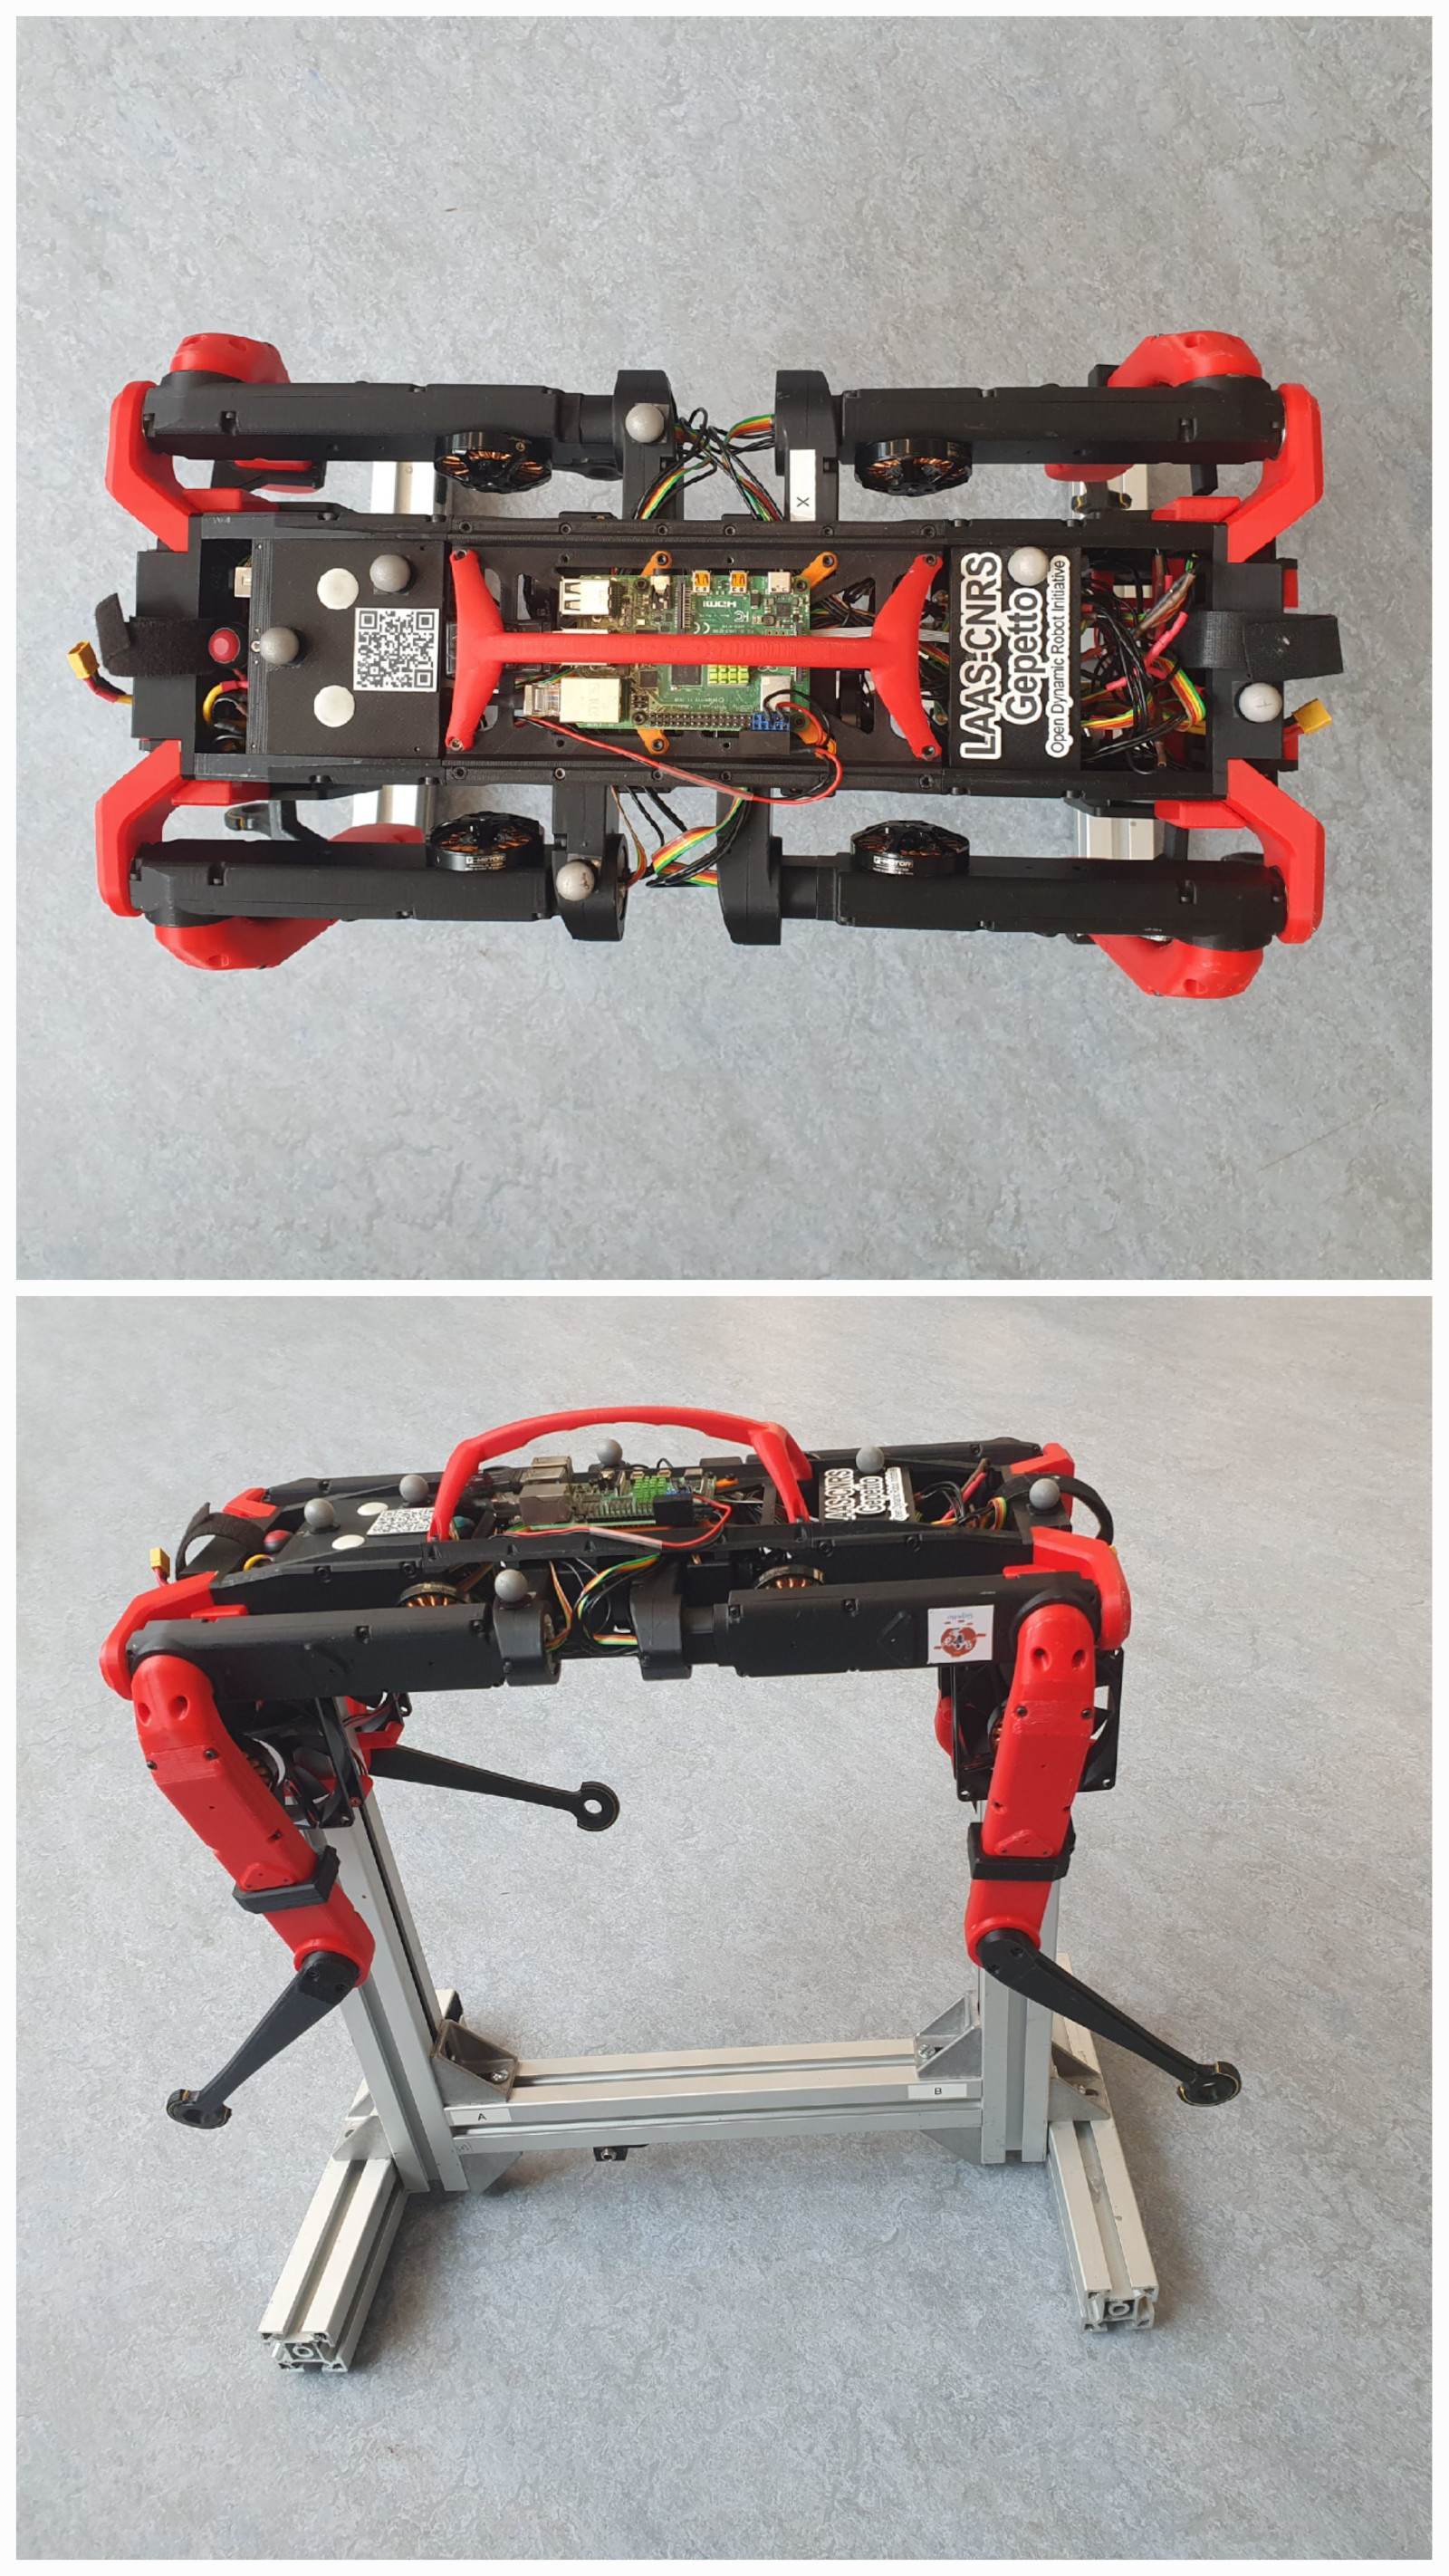
\includegraphics[width=\linewidth, angle=0, scale=0.5]{./images/Solo3.jpg}
  \caption{Solo 12}
\end{figure}

\subsection{What is Pinocchio ?}
Pinocchio is a library used for dynamical computations on robots. It has a large set of function for computing rotations, jacobians, forward kinematics, inverse kinematics, and so on. It is one of the, if not the one, most computationnally efficient library available for those tasks. From the user point of view, Pinocchio takes care of all the dirty physical equations in the background as long as you give it the right input. However, documentation is scarce. Version used was $2.7$. More information can be found at \url{https://github.com/stack-of-tasks/pinocchio}

\subsection{What is Croccodyl ?}

\subsection{What is ROS 2 ?}





\newpage




\section{Bibliography}

\printbibliography






\end{document}



